% Options for packages loaded elsewhere
\PassOptionsToPackage{unicode}{hyperref}
\PassOptionsToPackage{hyphens}{url}
%
\documentclass[
]{article}
\usepackage{amsmath,amssymb}
\usepackage{iftex}
\ifPDFTeX
  \usepackage[T1]{fontenc}
  \usepackage[utf8]{inputenc}
  \usepackage{textcomp} % provide euro and other symbols
\else % if luatex or xetex
  \usepackage{unicode-math} % this also loads fontspec
  \defaultfontfeatures{Scale=MatchLowercase}
  \defaultfontfeatures[\rmfamily]{Ligatures=TeX,Scale=1}
\fi
\usepackage{lmodern}
\ifPDFTeX\else
  % xetex/luatex font selection
\fi
% Use upquote if available, for straight quotes in verbatim environments
\IfFileExists{upquote.sty}{\usepackage{upquote}}{}
\IfFileExists{microtype.sty}{% use microtype if available
  \usepackage[]{microtype}
  \UseMicrotypeSet[protrusion]{basicmath} % disable protrusion for tt fonts
}{}
\makeatletter
\@ifundefined{KOMAClassName}{% if non-KOMA class
  \IfFileExists{parskip.sty}{%
    \usepackage{parskip}
  }{% else
    \setlength{\parindent}{0pt}
    \setlength{\parskip}{6pt plus 2pt minus 1pt}}
}{% if KOMA class
  \KOMAoptions{parskip=half}}
\makeatother
\usepackage{xcolor}
\usepackage[margin=1in]{geometry}
\usepackage{color}
\usepackage{fancyvrb}
\newcommand{\VerbBar}{|}
\newcommand{\VERB}{\Verb[commandchars=\\\{\}]}
\DefineVerbatimEnvironment{Highlighting}{Verbatim}{commandchars=\\\{\}}
% Add ',fontsize=\small' for more characters per line
\usepackage{framed}
\definecolor{shadecolor}{RGB}{248,248,248}
\newenvironment{Shaded}{\begin{snugshade}}{\end{snugshade}}
\newcommand{\AlertTok}[1]{\textcolor[rgb]{0.94,0.16,0.16}{#1}}
\newcommand{\AnnotationTok}[1]{\textcolor[rgb]{0.56,0.35,0.01}{\textbf{\textit{#1}}}}
\newcommand{\AttributeTok}[1]{\textcolor[rgb]{0.13,0.29,0.53}{#1}}
\newcommand{\BaseNTok}[1]{\textcolor[rgb]{0.00,0.00,0.81}{#1}}
\newcommand{\BuiltInTok}[1]{#1}
\newcommand{\CharTok}[1]{\textcolor[rgb]{0.31,0.60,0.02}{#1}}
\newcommand{\CommentTok}[1]{\textcolor[rgb]{0.56,0.35,0.01}{\textit{#1}}}
\newcommand{\CommentVarTok}[1]{\textcolor[rgb]{0.56,0.35,0.01}{\textbf{\textit{#1}}}}
\newcommand{\ConstantTok}[1]{\textcolor[rgb]{0.56,0.35,0.01}{#1}}
\newcommand{\ControlFlowTok}[1]{\textcolor[rgb]{0.13,0.29,0.53}{\textbf{#1}}}
\newcommand{\DataTypeTok}[1]{\textcolor[rgb]{0.13,0.29,0.53}{#1}}
\newcommand{\DecValTok}[1]{\textcolor[rgb]{0.00,0.00,0.81}{#1}}
\newcommand{\DocumentationTok}[1]{\textcolor[rgb]{0.56,0.35,0.01}{\textbf{\textit{#1}}}}
\newcommand{\ErrorTok}[1]{\textcolor[rgb]{0.64,0.00,0.00}{\textbf{#1}}}
\newcommand{\ExtensionTok}[1]{#1}
\newcommand{\FloatTok}[1]{\textcolor[rgb]{0.00,0.00,0.81}{#1}}
\newcommand{\FunctionTok}[1]{\textcolor[rgb]{0.13,0.29,0.53}{\textbf{#1}}}
\newcommand{\ImportTok}[1]{#1}
\newcommand{\InformationTok}[1]{\textcolor[rgb]{0.56,0.35,0.01}{\textbf{\textit{#1}}}}
\newcommand{\KeywordTok}[1]{\textcolor[rgb]{0.13,0.29,0.53}{\textbf{#1}}}
\newcommand{\NormalTok}[1]{#1}
\newcommand{\OperatorTok}[1]{\textcolor[rgb]{0.81,0.36,0.00}{\textbf{#1}}}
\newcommand{\OtherTok}[1]{\textcolor[rgb]{0.56,0.35,0.01}{#1}}
\newcommand{\PreprocessorTok}[1]{\textcolor[rgb]{0.56,0.35,0.01}{\textit{#1}}}
\newcommand{\RegionMarkerTok}[1]{#1}
\newcommand{\SpecialCharTok}[1]{\textcolor[rgb]{0.81,0.36,0.00}{\textbf{#1}}}
\newcommand{\SpecialStringTok}[1]{\textcolor[rgb]{0.31,0.60,0.02}{#1}}
\newcommand{\StringTok}[1]{\textcolor[rgb]{0.31,0.60,0.02}{#1}}
\newcommand{\VariableTok}[1]{\textcolor[rgb]{0.00,0.00,0.00}{#1}}
\newcommand{\VerbatimStringTok}[1]{\textcolor[rgb]{0.31,0.60,0.02}{#1}}
\newcommand{\WarningTok}[1]{\textcolor[rgb]{0.56,0.35,0.01}{\textbf{\textit{#1}}}}
\usepackage{longtable,booktabs,array}
\usepackage{calc} % for calculating minipage widths
% Correct order of tables after \paragraph or \subparagraph
\usepackage{etoolbox}
\makeatletter
\patchcmd\longtable{\par}{\if@noskipsec\mbox{}\fi\par}{}{}
\makeatother
% Allow footnotes in longtable head/foot
\IfFileExists{footnotehyper.sty}{\usepackage{footnotehyper}}{\usepackage{footnote}}
\makesavenoteenv{longtable}
\usepackage{graphicx}
\makeatletter
\newsavebox\pandoc@box
\newcommand*\pandocbounded[1]{% scales image to fit in text height/width
  \sbox\pandoc@box{#1}%
  \Gscale@div\@tempa{\textheight}{\dimexpr\ht\pandoc@box+\dp\pandoc@box\relax}%
  \Gscale@div\@tempb{\linewidth}{\wd\pandoc@box}%
  \ifdim\@tempb\p@<\@tempa\p@\let\@tempa\@tempb\fi% select the smaller of both
  \ifdim\@tempa\p@<\p@\scalebox{\@tempa}{\usebox\pandoc@box}%
  \else\usebox{\pandoc@box}%
  \fi%
}
% Set default figure placement to htbp
\def\fps@figure{htbp}
\makeatother
\setlength{\emergencystretch}{3em} % prevent overfull lines
\providecommand{\tightlist}{%
  \setlength{\itemsep}{0pt}\setlength{\parskip}{0pt}}
\setcounter{secnumdepth}{5}
\usepackage{booktabs}
\usepackage{longtable}
\usepackage{array}
\usepackage{multirow}
\usepackage{wrapfig}
\usepackage{float}
\usepackage{colortbl}
\usepackage{pdflscape}
\usepackage{tabu}
\usepackage{threeparttable}
\usepackage{threeparttablex}
\usepackage[normalem]{ulem}
\usepackage{makecell}
\usepackage{xcolor}
\usepackage{bookmark}
\IfFileExists{xurl.sty}{\usepackage{xurl}}{} % add URL line breaks if available
\urlstyle{same}
\hypersetup{
  pdftitle={Einfluss der Wettbewerbsstruktur auf Gehaltsniveaus im Data Science-Bereich:},
  hidelinks,
  pdfcreator={LaTeX via pandoc}}

\title{Einfluss der Wettbewerbsstruktur auf Gehaltsniveaus im Data
Science-Bereich:}
\usepackage{etoolbox}
\makeatletter
\providecommand{\subtitle}[1]{% add subtitle to \maketitle
  \apptocmd{\@title}{\par {\large #1 \par}}{}{}
}
\makeatother
\subtitle{Eine Social Network Analyse}
\author{}
\date{\vspace{-2.5em}}

\begin{document}
\maketitle

{
\setcounter{tocdepth}{3}
\tableofcontents
}
\newpage

\section{Einleitung}\label{einleitung}

\subsection{Requirements}\label{requirements}

Zunächst müssen die benötigten Bibliotheken installiert werden:

\begin{itemize}
\tightlist
\item
  \$ install.packages(``tidyverse'')
\item
  \$ install.packages(``igraph'')
\item
  \$ install.packages(``visNetwork'')
\item
  \$ install.packages(``dplyr'')
\item
  \$ install.packages(``tidyr'')
\item
  \$ install.packages(``kableExtra'')
\item
  \$ install.packages(``webshot'')
\item
  \$ install.packages(``knitr'')
\item
  \$ install.packages(``ggplot2'')
\item
  \$ install.packages(``RColorBrewer'')
\item
  \$ install.packages(``skimr'')
\end{itemize}

Und anschließend geladen werden:

\begin{Shaded}
\begin{Highlighting}[]
\FunctionTok{library}\NormalTok{(tidyverse)}
\FunctionTok{library}\NormalTok{(igraph)}
\FunctionTok{library}\NormalTok{(visNetwork)}
\FunctionTok{library}\NormalTok{(dplyr)}
\FunctionTok{library}\NormalTok{(tidyr)}
\FunctionTok{library}\NormalTok{(knitr)}
\FunctionTok{library}\NormalTok{(kableExtra)}
\FunctionTok{library}\NormalTok{(webshot)}
\FunctionTok{library}\NormalTok{(ggplot2)}
\FunctionTok{library}\NormalTok{(RColorBrewer)}
\FunctionTok{library}\NormalTok{(skimr)}
\end{Highlighting}
\end{Shaded}

\subsection{Motivation und
Zielsetzung}\label{motivation-und-zielsetzung}

In ihrem Artikel ``Data Scientist: The Sexiest Job of the 21st Century''
betonen Davenport und Patil, dass Data Scientists durch ihre Fähigkeiten
in Informatik, Statistik und ihr Fachwissen allgemein einen erheblichen
Mehrwert für Unternehmen schaffen.\footnote{Davenport, Patil 2012} Die
Fähigkeit, aus komplexen, unstrukturierten Daten wertvolle Erkenntnisse
zu gewinnen, macht Data Scientisten in vielen Branchen zu einer
unverzichtbaren Ressource.\footnote{Davenport, Patil 2012} Die Nutzung
ihrer Kompetenzen verschafft Unternehmen einen Wettbewerbsvorteil, da
sie datengetriebene Entscheidungen, Produktinnovationen und
Effizienzsteigerungen ermöglicht.\footnote{Davenport, Patil 2012}

Darüber ob Data Scientists immer noch the ``Sexiest Job'' des 21.
Jahrhunderts sind, lässt sich streiten. Fakt ist jedoch, dass die
Nachfrage nach Data Scientists in den letzten Jahren stark gestiegen ist
und vorraussichtlich immer weiter steigen wird. Dieser Trend ist auch in
den Google-Suchanfragen zu den Begriffen erkenntlich:\footnote{Google
  Trends, abgerufen am 30.10.2024}

\begin{Shaded}
\begin{Highlighting}[]
\FunctionTok{ggplot}\NormalTok{(data, }\FunctionTok{aes}\NormalTok{(}\AttributeTok{x =}\NormalTok{ Monat)) }\SpecialCharTok{+}
  \FunctionTok{geom\_line}\NormalTok{(}\FunctionTok{aes}\NormalTok{(}\AttributeTok{y =} \StringTok{\textasciigrave{}}\AttributeTok{data science}\StringTok{\textasciigrave{}}\NormalTok{, }\AttributeTok{color =} \StringTok{"data science"}\NormalTok{)) }\SpecialCharTok{+}
  \FunctionTok{geom\_line}\NormalTok{(}\FunctionTok{aes}\NormalTok{(}\AttributeTok{y =} \StringTok{\textasciigrave{}}\AttributeTok{data scientist}\StringTok{\textasciigrave{}}\NormalTok{, }\AttributeTok{color =} \StringTok{"data scientist"}\NormalTok{)) }\SpecialCharTok{+}
  \FunctionTok{labs}\NormalTok{(}\AttributeTok{title =} \StringTok{"Google Suchtrend für \textquotesingle{}data science\textquotesingle{} und \textquotesingle{}data scientist\textquotesingle{}"}\NormalTok{,}
       \AttributeTok{x =} \StringTok{"Datum"}\NormalTok{,}
       \AttributeTok{y =} \StringTok{"Interesse"}\NormalTok{,}
       \AttributeTok{color =} \StringTok{"Suchbegriff"}\NormalTok{) }\SpecialCharTok{+}
  \FunctionTok{theme\_minimal}\NormalTok{()}
\end{Highlighting}
\end{Shaded}

\pandocbounded{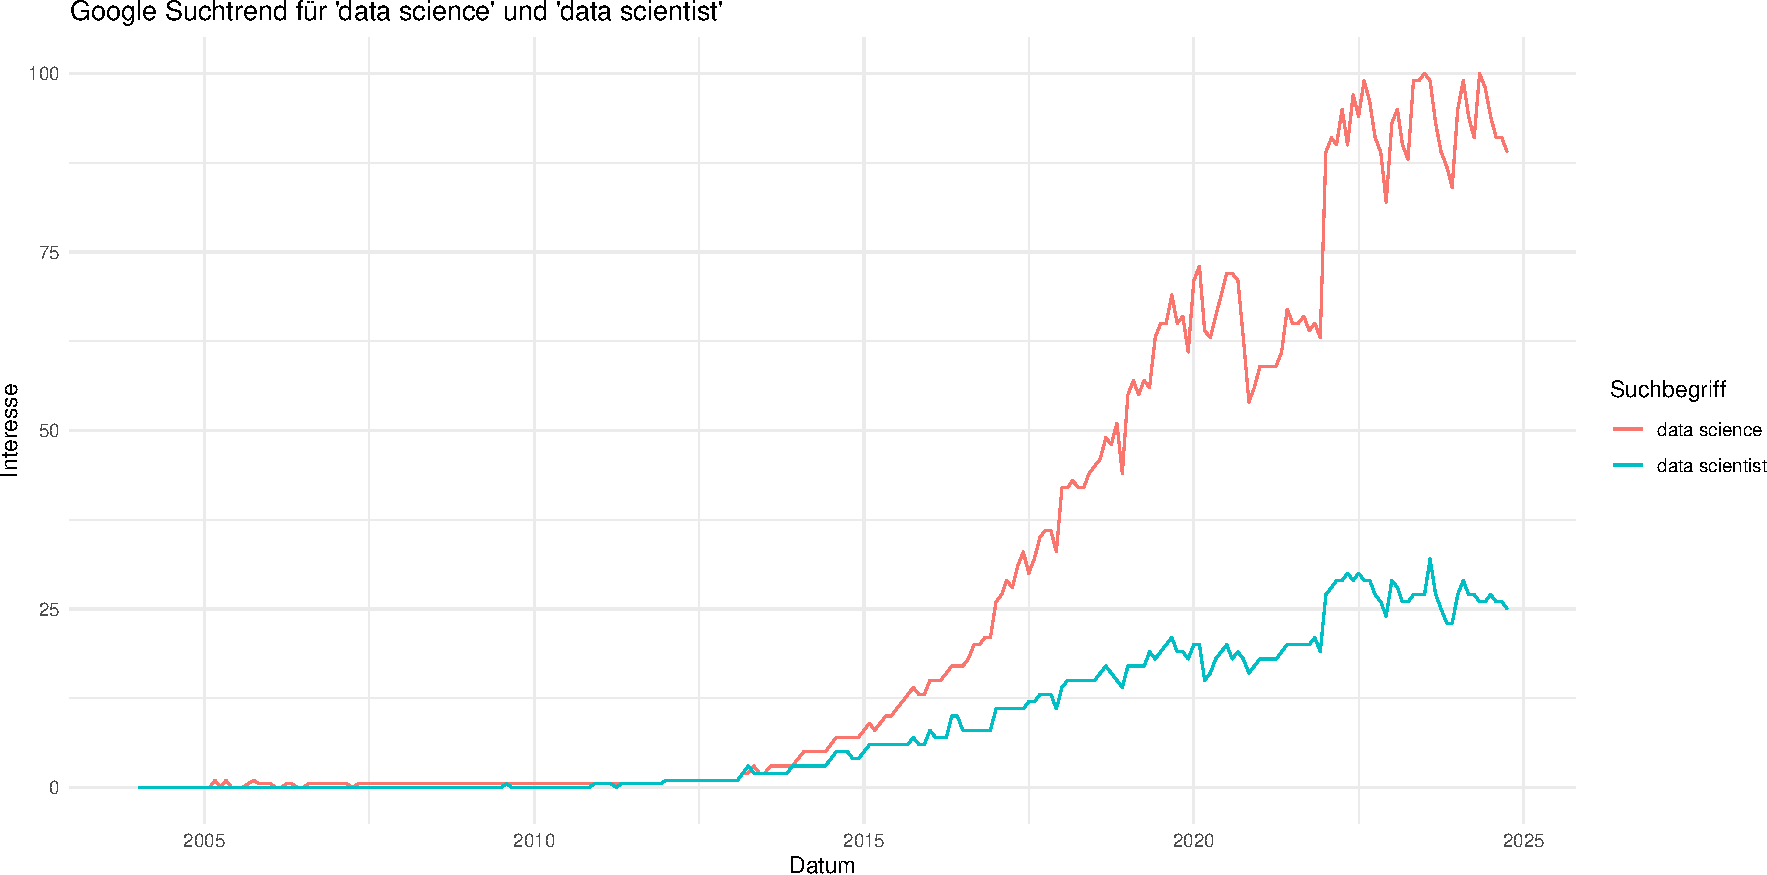
\includegraphics[keepaspectratio]{DataScience_files/figure-latex/unnamed-chunk-2-1.pdf}}

Das wachsende Interesse an Data Science stellt eine große Chance für
Arbeitnehmer dar. Ziel dieser Arbeit ist es einen Überblick über den
Data-Science-Jobmarkt zu geben, um Arbeitnehmern bei der Jobsuche zu
helfen und andererseits einen Überblick über die Gehälter und die Rolle
von Geographie und Wettbewerb bei Jobangeboten und Gehältern zu geben.

\subsection{Forschungsfrage}\label{forschungsfrage}

Im Rahmen der vorliegenden Arbeit wird die folgende Forschungsfrage
bearbeitet:

Inwiefern beeinflusst die geografische Nähe von Unternehmen das
Gehaltsniveau und die Verfügbarkeit von Data-Science-Jobs? Lässt sich
eine signifikante Variation der Einkommen innerhalb regionaler Cluster
feststellen, und wie kann diese durch Netzwerkzentralität erklärt
werden?

Zur Beantwortung dieser Forschungsfrage soll zudem analysiert werden,
inwiefern das Wettbewerbsumfeld zwischen Unternehmen die Gehaltsstruktur
im Bereich Data Science beeinflusst und welche Rolle zentrale
Unternehmen bei der Bestimmung des Gehaltsniveaus spielen.

\subsection{Datengrundlage}\label{datengrundlage}

Nachdem die Daten in Python extern als Vorbereitung aufbereitet wurden,
kann nun die Datengrundlage für diese Arbeit in R eingelesen werden.
Dabei wurde sich an
\url{https://www.kaggle.com/code/fahadrehman07/data-science-job-salary-prediction-glassdoor}
orientiert.

\subsubsection{CSV einlesen}\label{csv-einlesen}

\begin{Shaded}
\begin{Highlighting}[]
\NormalTok{data }\OtherTok{\textless{}{-}} \FunctionTok{read\_csv}\NormalTok{(}\StringTok{"data/Glassdoor\_DataScience\_Salary.csv"}\NormalTok{, }\AttributeTok{show\_col\_types =} \ConstantTok{FALSE}\NormalTok{)}
\end{Highlighting}
\end{Shaded}

Die vorliegende Arbeit basiert auf einem Datensatz von Kaggle, der
Informationen über Data Science Jobs in verschiedenen Unternehmen für
den US-amerikanischen Markt enthält. Der Datensatz umfasst 742 Zeilen
und 28 Spalten, was auf eine Anzahl von 742 verschiedenen Jobangeboten
hindeutet. Diese Anzahl ist kann für die Zwecke dieser Arbeit als
ausreichend zu betrachten, auch wenn eine höhere Zahl an Beobachtungen
möglicherweise zu präziseren Schlussfolgerungen geführt hätte.

Der Datensatz beruht auf Daten, die von Glassdoor extrahiert wurden,
eine für Stellenanzeigen und Unternehmensbewertung bekannte Website, und
bietet detaillierte Informationen über Data-Science-Jobs sowie deren
Gehälter. Der Datensatz beinhaltet wesentliche Informationen, darunter
Jobtitel, geschätzte Gehälter, Stellenbeschreibungen,
Unternehmensbewertungen sowie relevante Unternehmensdaten wie Standort,
Größe und Branche. Eine detaillierte Beschreibung dieser Daten erfolgt
im späteren Verlauf. Der Datensatz eignet sich in besonderem Maße für
den Zweck dieser Arbeit, aber auch für Analysen des Arbeitsmarktes,
beispielsweise zur Untersuchung von Gehaltstrends oder zur
Identifizierung der am besten bewerteten Unternehmen.

Der Datensatz umfasst konkret die folgenden Spalten:

\subsubsection{Erste Ansicht der Daten}\label{erste-ansicht-der-daten}

\begin{Shaded}
\begin{Highlighting}[]
\FunctionTok{head}\NormalTok{(data, }\DecValTok{5}\NormalTok{)}
\end{Highlighting}
\end{Shaded}

\begin{verbatim}
## # A tibble: 5 x 28
##   `Job Title` `Salary Estimate` `Job Description` Rating `Company Name` Location
##   <chr>                   <dbl> <chr>              <dbl> <chr>          <chr>   
## 1 Data Scien~              72   "Data Scientist\~    3.8 Tecolote Rese~ Albuque~
## 2 Healthcare~              87.5 "What You Will D~    3.4 University of~ Linthic~
## 3 Data Scien~              85   "KnowBe4, Inc. i~    4.8 KnowBe4        Clearwa~
## 4 Data Scien~              76.5 "*Organization a~    3.8 PNNL           Richlan~
## 5 Data Scien~             114.  "Data Scientist\~    2.9 Affinity Solu~ New Yor~
## # i 22 more variables: Headquarters <chr>, Size <chr>, Founded <dbl>,
## #   `Type of ownership` <chr>, Industry <chr>, Sector <chr>, Revenue <chr>,
## #   Competitors <chr>, Min_Salary <dbl>, Max_Salary <dbl>, State <chr>,
## #   `Same State` <dbl>, Age <dbl>, Python_yn <dbl>, `R Studio` <dbl>,
## #   Spark <dbl>, AWS_yn <dbl>, Excel_yn <dbl>, Job_simp <chr>, job_state <chr>,
## #   desc_len <dbl>, Num_comp <dbl>
\end{verbatim}

\begin{Shaded}
\begin{Highlighting}[]
\FunctionTok{spec}\NormalTok{(data)}
\end{Highlighting}
\end{Shaded}

\begin{verbatim}
## cols(
##   `Job Title` = col_character(),
##   `Salary Estimate` = col_double(),
##   `Job Description` = col_character(),
##   Rating = col_double(),
##   `Company Name` = col_character(),
##   Location = col_character(),
##   Headquarters = col_character(),
##   Size = col_character(),
##   Founded = col_double(),
##   `Type of ownership` = col_character(),
##   Industry = col_character(),
##   Sector = col_character(),
##   Revenue = col_character(),
##   Competitors = col_character(),
##   Min_Salary = col_double(),
##   Max_Salary = col_double(),
##   State = col_character(),
##   `Same State` = col_double(),
##   Age = col_double(),
##   Python_yn = col_double(),
##   `R Studio` = col_double(),
##   Spark = col_double(),
##   AWS_yn = col_double(),
##   Excel_yn = col_double(),
##   Job_simp = col_character(),
##   job_state = col_character(),
##   desc_len = col_double(),
##   Num_comp = col_double()
## )
\end{verbatim}

\begin{Shaded}
\begin{Highlighting}[]
\CommentTok{\# Erstellen eine schönen Zusammenfassung des Datensatzes}
\FunctionTok{skim}\NormalTok{(data)}
\end{Highlighting}
\end{Shaded}

\begin{longtable}[]{@{}ll@{}}
\caption{Data summary}\tabularnewline
\toprule\noalign{}
\endfirsthead
\endhead
\bottomrule\noalign{}
\endlastfoot
Name & data \\
Number of rows & 742 \\
Number of columns & 28 \\
\_\_\_\_\_\_\_\_\_\_\_\_\_\_\_\_\_\_\_\_\_\_\_ & \\
Column type frequency: & \\
character & 14 \\
numeric & 14 \\
\_\_\_\_\_\_\_\_\_\_\_\_\_\_\_\_\_\_\_\_\_\_\_\_ & \\
Group variables & None \\
\end{longtable}

\textbf{Variable type: character}

\begin{longtable}[]{@{}
  >{\raggedright\arraybackslash}p{(\linewidth - 14\tabcolsep) * \real{0.2308}}
  >{\raggedleft\arraybackslash}p{(\linewidth - 14\tabcolsep) * \real{0.1282}}
  >{\raggedleft\arraybackslash}p{(\linewidth - 14\tabcolsep) * \real{0.1795}}
  >{\raggedleft\arraybackslash}p{(\linewidth - 14\tabcolsep) * \real{0.0513}}
  >{\raggedleft\arraybackslash}p{(\linewidth - 14\tabcolsep) * \real{0.0769}}
  >{\raggedleft\arraybackslash}p{(\linewidth - 14\tabcolsep) * \real{0.0769}}
  >{\raggedleft\arraybackslash}p{(\linewidth - 14\tabcolsep) * \real{0.1154}}
  >{\raggedleft\arraybackslash}p{(\linewidth - 14\tabcolsep) * \real{0.1410}}@{}}
\toprule\noalign{}
\begin{minipage}[b]{\linewidth}\raggedright
skim\_variable
\end{minipage} & \begin{minipage}[b]{\linewidth}\raggedleft
n\_missing
\end{minipage} & \begin{minipage}[b]{\linewidth}\raggedleft
complete\_rate
\end{minipage} & \begin{minipage}[b]{\linewidth}\raggedleft
min
\end{minipage} & \begin{minipage}[b]{\linewidth}\raggedleft
max
\end{minipage} & \begin{minipage}[b]{\linewidth}\raggedleft
empty
\end{minipage} & \begin{minipage}[b]{\linewidth}\raggedleft
n\_unique
\end{minipage} & \begin{minipage}[b]{\linewidth}\raggedleft
whitespace
\end{minipage} \\
\midrule\noalign{}
\endhead
\bottomrule\noalign{}
\endlastfoot
Job Title & 0 & 1 & 9 & 98 & 0 & 264 & 0 \\
Job Description & 0 & 1 & 407 & 10051 & 0 & 463 & 0 \\
Company Name & 0 & 1 & 2 & 51 & 0 & 343 & 0 \\
Location & 0 & 1 & 8 & 33 & 0 & 200 & 0 \\
Headquarters & 0 & 1 & 2 & 26 & 0 & 198 & 0 \\
Size & 0 & 1 & 2 & 23 & 0 & 9 & 0 \\
Type of ownership & 0 & 1 & 2 & 30 & 0 & 11 & 0 \\
Industry & 0 & 1 & 2 & 40 & 0 & 60 & 0 \\
Sector & 0 & 1 & 2 & 34 & 0 & 25 & 0 \\
Revenue & 0 & 1 & 2 & 32 & 0 & 14 & 0 \\
Competitors & 0 & 1 & 2 & 92 & 0 & 128 & 0 \\
State & 0 & 1 & 2 & 11 & 0 & 38 & 0 \\
Job\_simp & 0 & 1 & 2 & 14 & 0 & 7 & 0 \\
job\_state & 0 & 1 & 2 & 2 & 0 & 37 & 0 \\
\end{longtable}

\textbf{Variable type: numeric}

\begin{longtable}[]{@{}
  >{\raggedright\arraybackslash}p{(\linewidth - 20\tabcolsep) * \real{0.1684}}
  >{\raggedleft\arraybackslash}p{(\linewidth - 20\tabcolsep) * \real{0.1053}}
  >{\raggedleft\arraybackslash}p{(\linewidth - 20\tabcolsep) * \real{0.1474}}
  >{\raggedleft\arraybackslash}p{(\linewidth - 20\tabcolsep) * \real{0.0842}}
  >{\raggedleft\arraybackslash}p{(\linewidth - 20\tabcolsep) * \real{0.0842}}
  >{\raggedleft\arraybackslash}p{(\linewidth - 20\tabcolsep) * \real{0.0632}}
  >{\raggedleft\arraybackslash}p{(\linewidth - 20\tabcolsep) * \real{0.0737}}
  >{\raggedleft\arraybackslash}p{(\linewidth - 20\tabcolsep) * \real{0.0737}}
  >{\raggedleft\arraybackslash}p{(\linewidth - 20\tabcolsep) * \real{0.0737}}
  >{\raggedleft\arraybackslash}p{(\linewidth - 20\tabcolsep) * \real{0.0632}}
  >{\raggedright\arraybackslash}p{(\linewidth - 20\tabcolsep) * \real{0.0632}}@{}}
\toprule\noalign{}
\begin{minipage}[b]{\linewidth}\raggedright
skim\_variable
\end{minipage} & \begin{minipage}[b]{\linewidth}\raggedleft
n\_missing
\end{minipage} & \begin{minipage}[b]{\linewidth}\raggedleft
complete\_rate
\end{minipage} & \begin{minipage}[b]{\linewidth}\raggedleft
mean
\end{minipage} & \begin{minipage}[b]{\linewidth}\raggedleft
sd
\end{minipage} & \begin{minipage}[b]{\linewidth}\raggedleft
p0
\end{minipage} & \begin{minipage}[b]{\linewidth}\raggedleft
p25
\end{minipage} & \begin{minipage}[b]{\linewidth}\raggedleft
p50
\end{minipage} & \begin{minipage}[b]{\linewidth}\raggedleft
p75
\end{minipage} & \begin{minipage}[b]{\linewidth}\raggedleft
p100
\end{minipage} & \begin{minipage}[b]{\linewidth}\raggedright
hist
\end{minipage} \\
\midrule\noalign{}
\endhead
\bottomrule\noalign{}
\endlastfoot
Salary Estimate & 0 & 1 & 100.63 & 38.86 & 13.5 & 73.5 & 97.5 & 122.5 &
254 & ▂▇▅▁▁ \\
Rating & 0 & 1 & 3.62 & 0.80 & -1.0 & 3.3 & 3.7 & 4.0 & 5 & ▁▁▁▇▅ \\
Founded & 0 & 1 & 1837.15 & 497.18 & -1.0 & 1939.0 & 1988.0 & 2007.0 &
2019 & ▁▁▁▁▇ \\
Min\_Salary & 0 & 1 & 74.72 & 30.98 & 15.0 & 52.0 & 69.5 & 91.0 & 202 &
▅▇▃▁▁ \\
Max\_Salary & 0 & 1 & 127.18 & 46.91 & 16.0 & 96.0 & 124.0 & 155.0 & 306
& ▂▇▆▂▁ \\
Same State & 0 & 1 & 0.56 & 0.50 & 0.0 & 0.0 & 1.0 & 1.0 & 1 & ▆▁▁▁▇ \\
Age & 0 & 1 & 49.39 & 53.96 & -1.0 & 14.0 & 27.0 & 62.0 & 279 & ▇▂▁▁▁ \\
Python\_yn & 0 & 1 & 0.53 & 0.50 & 0.0 & 0.0 & 1.0 & 1.0 & 1 & ▇▁▁▁▇ \\
R Studio & 0 & 1 & 0.00 & 0.05 & 0.0 & 0.0 & 0.0 & 0.0 & 1 & ▇▁▁▁▁ \\
Spark & 0 & 1 & 0.23 & 0.42 & 0.0 & 0.0 & 0.0 & 0.0 & 1 & ▇▁▁▁▂ \\
AWS\_yn & 0 & 1 & 0.24 & 0.43 & 0.0 & 0.0 & 0.0 & 0.0 & 1 & ▇▁▁▁▂ \\
Excel\_yn & 0 & 1 & 0.52 & 0.50 & 0.0 & 0.0 & 1.0 & 1.0 & 1 & ▇▁▁▁▇ \\
desc\_len & 0 & 1 & 3869.55 & 1521.50 & 407.0 & 2801.0 & 3731.0 & 4740.0
& 10051 & ▂▇▅▁▁ \\
Num\_comp & 0 & 1 & 1.05 & 1.38 & 0.0 & 0.0 & 0.0 & 3.0 & 4 & ▇▁▁▃▁ \\
\end{longtable}

Im Folgenden wird eine Übersicht der wesentlichen Spalten präsentiert:

\begin{itemize}
\tightlist
\item
  \texttt{Job\ Title}: Die Berufsbezeichnung, sie gibt Aufschluss über
  die Tätigkeit.
\item
  \texttt{Salary\ Estimate}: Die geschätzte Gehalt, in tausend Dollar
  pro Jahr. Es basiert auf dem Durchschnitt von dem minimalen und
  maximalen Gehalt.
\item
  \texttt{Job\ Description}, \texttt{Job\_simp}: Die Beschreibung der
  Stelle, die Aufgaben und Anforderungen enthält. Auch die vereinfachte
  Version der Berufsbezeichnung.
\item
  \texttt{Rating}: Die Bewertung des Unternehmens, sie weist eine
  Spannbreite von 1 bis 5 auf, wobei die Bewertung ``-1'' bei jeder
  Spalte für fehlende Bewertungen steht.
\item
  \texttt{Company\ Name}, \texttt{Location}, \texttt{Headquarters},
  \texttt{Size}, \texttt{Founded}: Unternehmensbezogene Daten wie Name,
  Standort, Sitz, Größe und Gründungsjahr des Unternehmens.
\item
  \texttt{Type\ of\ ownership}, \texttt{Industry}, \texttt{Sector},
  \texttt{Revenue}: Weitere Unternehmensmerkmale, diese umfassen die
  Eigentumsart, die Branche, den Sektor sowie die Einnahmen.
\item
  \texttt{Competitors}: Die Wettbewerber des Unternehmens, die im
  Zusammenhang dieser Arbeit von besonderer Bedeutung sind.
\item
  Skills (\texttt{Python\_yn}, \texttt{R\ Studio}, \texttt{Spark},
  \texttt{AWS\_yn}, \texttt{Excel\_yn}): Spalten, aus denen hervorgeht,
  ob die betreffende Kompetenz in der Stellenbeschreibung verlangt wird
  (0 = nein, 1 = ja).
\item
  \texttt{Min\_salary}, \texttt{Max\_salary}: Minimale und maximale
  Gehaltsschätzungen.
\item
  \texttt{State}, \texttt{Same\ State}, \texttt{job\_state},
  \texttt{Age}, \texttt{desc\_len}, \texttt{Num\_comp}: Zusätzliche
  Informationen wie Standort der Stelle, Alter des Unternehmens, Länge
  der Stellenbeschreibung und Anzahl der Mitbewerber.
\end{itemize}

Es zeigt sich, dass eine Vielzahl von Spalten für die vorliegende
Untersuchung irrelevant ist. Infolgedessen werden in einem späteren Teil
der Arbeit irrelevante Spalten, wie beispielsweise die Kenntnisse in
Python, R Studio, Spark und ähnlichen Programmen, welche ursprünglich
aus der Jobbeschreibung extrahiert wurden, entfernt.

Nachdem die Daten in Python mit Hilfe von Pandas bereinigt, ergänzt und
bearbeitet wurden, können sie nun in R eingelesen werden.

Im Folgenden wird eine erste Betrachtung der Daten vorgenommen. Zu
diesem Zweck werden die Jobs in New York nach ihren jeweiligen
Vergütungen geordnet und in Form eines Balkendiagramms dargestellt.

\begin{Shaded}
\begin{Highlighting}[]
\CommentTok{\# Filterung der Daten für New York}
\NormalTok{data\_ny }\OtherTok{\textless{}{-}}\NormalTok{ data }\SpecialCharTok{\%\textgreater{}\%}
  \FunctionTok{filter}\NormalTok{(State }\SpecialCharTok{==} \StringTok{"NY"}\NormalTok{)}

\CommentTok{\# Durchschnittsgehalt nach Berufsbezeichnung}
\NormalTok{avg\_salary\_by\_job\_ny }\OtherTok{\textless{}{-}}\NormalTok{ data\_ny }\SpecialCharTok{\%\textgreater{}\%}
  \FunctionTok{group\_by}\NormalTok{(}\StringTok{\textasciigrave{}}\AttributeTok{Job Title}\StringTok{\textasciigrave{}}\NormalTok{) }\SpecialCharTok{\%\textgreater{}\%}
  \FunctionTok{summarise}\NormalTok{(}\AttributeTok{Average\_Salary =} \FunctionTok{mean}\NormalTok{(}\StringTok{\textasciigrave{}}\AttributeTok{Salary Estimate}\StringTok{\textasciigrave{}}\NormalTok{, }\AttributeTok{na.rm =} \ConstantTok{TRUE}\NormalTok{)) }\SpecialCharTok{\%\textgreater{}\%}
  \FunctionTok{arrange}\NormalTok{(}\FunctionTok{desc}\NormalTok{(Average\_Salary))}

\CommentTok{\# Bar Plot}
\FunctionTok{ggplot}\NormalTok{(avg\_salary\_by\_job\_ny,}
       \FunctionTok{aes}\NormalTok{(}\AttributeTok{x =} \FunctionTok{reorder}\NormalTok{(}\StringTok{\textasciigrave{}}\AttributeTok{Job Title}\StringTok{\textasciigrave{}}\NormalTok{, Average\_Salary), }\AttributeTok{y =}\NormalTok{ Average\_Salary)) }\SpecialCharTok{+}
  \FunctionTok{geom\_bar}\NormalTok{(}\AttributeTok{stat =} \StringTok{"identity"}\NormalTok{) }\SpecialCharTok{+}
  \FunctionTok{coord\_flip}\NormalTok{() }\SpecialCharTok{+}
  \FunctionTok{labs}\NormalTok{(}\AttributeTok{title =} \StringTok{"Average Salary by Job Title in NY"}\NormalTok{,}
       \AttributeTok{x =} \StringTok{"Job Title"}\NormalTok{,}
       \AttributeTok{y =} \StringTok{"Average Salary"}\NormalTok{) }\SpecialCharTok{+}
  \FunctionTok{theme\_minimal}\NormalTok{() }\SpecialCharTok{+}
  \FunctionTok{theme}\NormalTok{(}
    \AttributeTok{axis.title =} \FunctionTok{element\_text}\NormalTok{(}\AttributeTok{size =} \DecValTok{14}\NormalTok{),}
    \AttributeTok{axis.text =} \FunctionTok{element\_text}\NormalTok{(}\AttributeTok{size =} \DecValTok{12}\NormalTok{),}
    \AttributeTok{plot.title =} \FunctionTok{element\_text}\NormalTok{(}\AttributeTok{size =} \DecValTok{16}\NormalTok{, }\AttributeTok{face =} \StringTok{"bold"}\NormalTok{)}
\NormalTok{  )}
\end{Highlighting}
\end{Shaded}

\pandocbounded{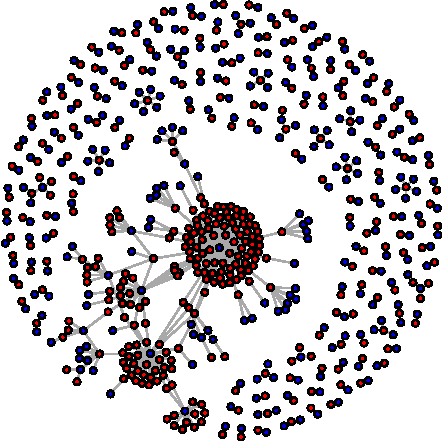
\includegraphics[keepaspectratio]{DataScience_files/figure-latex/unnamed-chunk-5-1.pdf}}
todo \ldots{} Insights aus dem Plot ziehen

Da die Datengrundlage nicht in einem igraph-Objekt vorliegt und
ungerichtet ist, ist es notwendig Knoten, Kanten sowie relevante
Attribute wie beispielsweise Gewichtungen zu definieren, um überhaupt
Netzwerkvisualisierungen in R durchführen zu können. Doch dazu mehr im
nächsten Kapitel.

\newpage

\section{Analysestrategie}\label{analysestrategie}

\begin{enumerate}
\def\labelenumi{\arabic{enumi}.}
\tightlist
\item
  Geografisches Netzwerk
\end{enumerate}

Das Ziel besteht in der Erstellung eines Netzwerkes, welches auf der
räumlichen Nähe von Unternehmen basiert. Auf diese Weise soll untersucht
werden, inwiefern regional bedingte Faktoren die Gehälter beeinflussen.
Die Bildung von Kanten erfolgt nach dem Kriterium der räumlichen Nähe.
Dabei werden Unternehmen, die im gleichen Ort angesiedelt sind, durch
Kanten verbunden.

\begin{enumerate}
\def\labelenumi{\arabic{enumi}.}
\setcounter{enumi}{1}
\tightlist
\item
  Wettbewerbsnetzwerk
\end{enumerate}

Die vorliegende Untersuchung zielt darauf ab, den Einfluss des
Wettbewerbs auf die Gestaltung von Gehaltsstrukturen zu analysieren.
Dazu werden die Beziehungen zwischen konkurrierenden Unternehmen als
Netzwerk dargestellt. Die Bildung von Kanten durch Konkurrenzen erfolgt
wie folgt: Die in der Spalte ``Competitors'' gelisteten Unternehmen
werden als Knoten verbunden. In Bezug auf die Gewichtung sind
verschiedene Optionen denkbar. Beispielsweise könnte die direkte
Konkurrenz mit dem Wert ``1'' und die indirekte Konkurrenz mit dem Wert
``0,5'' bewertet werden. Dabei würde die indirekte Konkurrenz eine
Branche umfassen, in der das Unternehmen zwar nicht als direkter
Konkurrent aufgeführt ist, jedoch potenziell in Konkurrenz stehen
könnte. Im Rahmen der Netzwerkmetriken erfolgt eine Analyse der
folgenden Aspekte: Im Rahmen der Analyse von hierarchischen Beziehungen
und unterschiedlichen Zentralitäten erfolgt eine Untersuchung der
Wichtigkeit eines Unternehmens im Wettbewerbsnetzwerk sowie der
Gehaltshöhen in Relation zur Konkurrenz.

\begin{enumerate}
\def\labelenumi{\arabic{enumi}.}
\setcounter{enumi}{2}
\tightlist
\item
  Vergleich der Gehälter innerhalb der Netzwerke
\end{enumerate}

Im Rahmen der Analyse werden die Gehälter innerhalb der beiden Netzwerke
miteinander verglichen. Ziel ist die Identifikation von Unternehmen, die
zentral in einem der beiden Netzwerke liegen, und solchen, die am Rand
oder isoliert sind, um festzustellen, ob die zentralen Unternehmen
höhere Gehälter anbieten. Zur Durchführung des Gehaltsvergleichs werden
Korrelationen zwischen dem Gehalt und verschiedenen Zentralitätsmaßen
innerhalb der geografischen und wettbewerbsbezogenen Netzwerke
herangezogen. Darüber hinaus werden Cluster-Analysen durchgeführt, um
Unternehmen, die geografisch und wettbewerbsbedingt vernetzt sind,
miteinander zu vergleichen.

\begin{enumerate}
\def\labelenumi{\arabic{enumi}.}
\setcounter{enumi}{3}
\tightlist
\item
  Zusammenführung und Vergleich der Netzwerke
\end{enumerate}

Im Rahmen der Zusammenführung und des Vergleichs der Netzwerke erfolgt
eine Gegenüberstellung der jeweiligen Strukturen, um etwaige
Gemeinsamkeiten und Unterschiede zu identifizieren. Das Ziel dieser
Untersuchung besteht in der Analyse der Interaktion beider Netzwerke
sowie der Identifikation von Regionen, in denen eine besonders hohe
Gehaltskonkurrenz zu beobachten ist. Im Rahmen des Vergleichs der
Netzwerke hinsichtlich der Gehälter und des Wettbewerbs erfolgt zunächst
eine Gegenüberstellung der Gehaltsverteilung in sogenannten
``Hotspot-Regionen'' und geografisch isolierten Regionen. Darüber hinaus
werden gemeinsame Unternehmen in beiden Netzwerken sowie die
Gehaltsstrukturen innerhalb der Überschneidungsbereiche analysiert.

\newpage

\section{Analyse}\label{analyse}

\subsection{Datenbereinigung}\label{datenbereinigung}

\subsubsection{Bereinigung für die geografische
Analyse}\label{bereinigung-fuxfcr-die-geografische-analyse}

Bei der Durchsicht des Datensatzes viel auf, dass die Spalten ``Same
State'' und ``job\_state'' von der Logik her ähnlich sind. Dies soll nun
näher unterucht werden, um spätere Fehler vorzubeugen, vor allem bei den
geografischen Netzwerken vorzubeugen.

\begin{Shaded}
\begin{Highlighting}[]
\CommentTok{\# Auswahl der "State" und "job\_state" Spalten}
\NormalTok{selected\_data }\OtherTok{\textless{}{-}}\NormalTok{ data }\SpecialCharTok{\%\textgreater{}\%}
  \FunctionTok{select}\NormalTok{(State, job\_state)}

\CommentTok{\# Heading der ausgewählten Spalten}
\FunctionTok{head}\NormalTok{(selected\_data, }\DecValTok{15}\NormalTok{)}
\end{Highlighting}
\end{Shaded}

\begin{verbatim}
## # A tibble: 15 x 2
##    State job_state
##    <chr> <chr>    
##  1 NM    NM       
##  2 MD    MD       
##  3 FL    FL       
##  4 WA    WA       
##  5 NY    NY       
##  6 TX    TX       
##  7 MD    MD       
##  8 CA    CA       
##  9 NY    NY       
## 10 NY    NY       
## 11 CA    CA       
## 12 VA    VA       
## 13 TX    TX       
## 14 WA    WA       
## 15 MA    MA
\end{verbatim}

Sieht so aus, als wäre beide Spalten identisch. Dies soll jedoch zur
Probe gestellt werden:

\begin{Shaded}
\begin{Highlighting}[]
\ControlFlowTok{if}\NormalTok{ (}\FunctionTok{all}\NormalTok{(selected\_data}\SpecialCharTok{$}\NormalTok{State }\SpecialCharTok{==}\NormalTok{ selected\_data}\SpecialCharTok{$}\NormalTok{job\_state, }\AttributeTok{na.rm =} \ConstantTok{TRUE}\NormalTok{)) \{}
  \FunctionTok{print}\NormalTok{(}\StringTok{"Alle Werte in \textquotesingle{}State\textquotesingle{} und \textquotesingle{}job\_state\textquotesingle{} sind identisch."}\NormalTok{)}
\NormalTok{\} }\ControlFlowTok{else}\NormalTok{ \{}
  \FunctionTok{print}\NormalTok{(}\StringTok{"Es gibt Unterschiede zwischen \textquotesingle{}State\textquotesingle{} und \textquotesingle{}job\_state\textquotesingle{}."}\NormalTok{)}
\NormalTok{\}}
\end{Highlighting}
\end{Shaded}

\begin{verbatim}
## [1] "Es gibt Unterschiede zwischen 'State' und 'job_state'."
\end{verbatim}

Jedoch trügt der Schein, da es Unterschiede gibt.

\begin{Shaded}
\begin{Highlighting}[]
\CommentTok{\# Auswahl der Zeilen, in denen "State" und "job\_state" unterschiedlich sind}
\NormalTok{different\_states }\OtherTok{\textless{}{-}}\NormalTok{ selected\_data }\SpecialCharTok{\%\textgreater{}\%}
  \FunctionTok{filter}\NormalTok{(State }\SpecialCharTok{!=}\NormalTok{ job\_state)}

\FunctionTok{print}\NormalTok{(different\_states, }\AttributeTok{n =} \ConstantTok{Inf}\NormalTok{)}
\end{Highlighting}
\end{Shaded}

\begin{verbatim}
## # A tibble: 1 x 2
##   State       job_state
##   <chr>       <chr>    
## 1 Los Angeles CA
\end{verbatim}

Es fällt auf, das LA und Los Angeles nicht einheitlich verwendet werden.
Außerdem ist Los Angeles kein eigener Bundesstaat, sonder ein Teil von
Kalifornien(CA). Dies soll nun korrigiert werden.

Außerdem sollte bei weieren Vorgehen beachtet werden, dass Werte wie
``Na'' oder ``-1'' vor den Analysen entfernt werden sollten.

\begin{Shaded}
\begin{Highlighting}[]
\CommentTok{\# Ersetzen von "Los Angeles" durch "LA" und "LA" durch "CA"}
\NormalTok{data }\OtherTok{\textless{}{-}}\NormalTok{ data }\SpecialCharTok{\%\textgreater{}\%}
  \FunctionTok{mutate}\NormalTok{(}\AttributeTok{State =} \FunctionTok{ifelse}\NormalTok{(State }\SpecialCharTok{==} \StringTok{"Los Angeles"}\NormalTok{, }\StringTok{"LA"}\NormalTok{, State),}
         \AttributeTok{job\_state =} \FunctionTok{ifelse}\NormalTok{(job\_state }\SpecialCharTok{==} \StringTok{"Los Angeles"}\NormalTok{, }\StringTok{"LA"}\NormalTok{, job\_state))}

\NormalTok{data }\OtherTok{\textless{}{-}}\NormalTok{ data }\SpecialCharTok{\%\textgreater{}\%}
  \FunctionTok{mutate}\NormalTok{(}\AttributeTok{State =} \FunctionTok{ifelse}\NormalTok{(State }\SpecialCharTok{==} \StringTok{"LA"}\NormalTok{, }\StringTok{"CA"}\NormalTok{, State),}
         \AttributeTok{job\_state =} \FunctionTok{ifelse}\NormalTok{(job\_state }\SpecialCharTok{==} \StringTok{"LA"}\NormalTok{, }\StringTok{"CA"}\NormalTok{, job\_state))}

\CommentTok{\# Erneute Überprüfung}
\NormalTok{selected\_data }\OtherTok{\textless{}{-}}\NormalTok{ data }\SpecialCharTok{\%\textgreater{}\%}
  \FunctionTok{select}\NormalTok{(State, job\_state)}

\ControlFlowTok{if}\NormalTok{ (}\FunctionTok{all}\NormalTok{(selected\_data}\SpecialCharTok{$}\NormalTok{State }\SpecialCharTok{==}\NormalTok{ selected\_data}\SpecialCharTok{$}\NormalTok{job\_state, }\AttributeTok{na.rm =} \ConstantTok{TRUE}\NormalTok{)) \{}
  \FunctionTok{print}\NormalTok{(}\StringTok{"Alle Werte in \textquotesingle{}State\textquotesingle{} und \textquotesingle{}job\_state\textquotesingle{} sind identisch."}\NormalTok{)}
\NormalTok{\} }\ControlFlowTok{else}\NormalTok{ \{}
  \FunctionTok{print}\NormalTok{(}\StringTok{"Es gibt Unterschiede zwischen \textquotesingle{}State\textquotesingle{} und \textquotesingle{}job\_state\textquotesingle{}."}\NormalTok{)}
\NormalTok{\}}
\end{Highlighting}
\end{Shaded}

\begin{verbatim}
## [1] "Alle Werte in 'State' und 'job_state' sind identisch."
\end{verbatim}

\subsubsection{Überprüfung auf weitere fehlende
Werte}\label{uxfcberpruxfcfung-auf-weitere-fehlende-werte}

\begin{Shaded}
\begin{Highlighting}[]
\CommentTok{\# Überprüfen auf NA{-}Werte}
\NormalTok{na\_counts }\OtherTok{\textless{}{-}} \FunctionTok{colSums}\NormalTok{(}\FunctionTok{is.na}\NormalTok{(data))}

\CommentTok{\# Anzahl der NA{-}Werte pro Spalte:}
\FunctionTok{print}\NormalTok{(na\_counts)}
\end{Highlighting}
\end{Shaded}

\begin{verbatim}
##         Job Title   Salary Estimate   Job Description            Rating 
##                 0                 0                 0                 0 
##      Company Name          Location      Headquarters              Size 
##                 0                 0                 0                 0 
##           Founded Type of ownership          Industry            Sector 
##                 0                 0                 0                 0 
##           Revenue       Competitors        Min_Salary        Max_Salary 
##                 0                 0                 0                 0 
##             State        Same State               Age         Python_yn 
##                 0                 0                 0                 0 
##          R Studio             Spark            AWS_yn          Excel_yn 
##                 0                 0                 0                 0 
##          Job_simp         job_state          desc_len          Num_comp 
##                 0                 0                 0                 0
\end{verbatim}

\begin{Shaded}
\begin{Highlighting}[]
\CommentTok{\# Überprüfen auf "na"{-}Werte (kleingeschrieben)}
\NormalTok{na\_string\_counts }\OtherTok{\textless{}{-}} \FunctionTok{sapply}\NormalTok{(data, }\ControlFlowTok{function}\NormalTok{(x) }\FunctionTok{sum}\NormalTok{(}\FunctionTok{tolower}\NormalTok{(x) }\SpecialCharTok{==} \StringTok{"na"}\NormalTok{, }\AttributeTok{na.rm =} \ConstantTok{TRUE}\NormalTok{))}

\CommentTok{\# Anzahl der "na"{-}Werte pro Spalte:}
\FunctionTok{print}\NormalTok{(na\_string\_counts)}
\end{Highlighting}
\end{Shaded}

\begin{verbatim}
##         Job Title   Salary Estimate   Job Description            Rating 
##                 0                 0                 0                 0 
##      Company Name          Location      Headquarters              Size 
##                 0                 0                 0                 0 
##           Founded Type of ownership          Industry            Sector 
##                 0                 0                 0                 0 
##           Revenue       Competitors        Min_Salary        Max_Salary 
##                 0                 0                 0                 0 
##             State        Same State               Age         Python_yn 
##                 0                 0                 0                 0 
##          R Studio             Spark            AWS_yn          Excel_yn 
##                 0                 0                 0                 0 
##          Job_simp         job_state          desc_len          Num_comp 
##               184                 0                 0                 0
\end{verbatim}

\begin{Shaded}
\begin{Highlighting}[]
\CommentTok{\# Überprüfen auf {-}1{-}Werte}
\NormalTok{neg\_one\_counts }\OtherTok{\textless{}{-}} \FunctionTok{sapply}\NormalTok{(data, }\ControlFlowTok{function}\NormalTok{(x) }\FunctionTok{sum}\NormalTok{(x }\SpecialCharTok{==} \SpecialCharTok{{-}}\DecValTok{1}\NormalTok{, }\AttributeTok{na.rm =} \ConstantTok{TRUE}\NormalTok{))}

\CommentTok{\# Anzahl der {-}1 Werte in der Spalte Competitors}
\FunctionTok{print}\NormalTok{(neg\_one\_counts)}
\end{Highlighting}
\end{Shaded}

\begin{verbatim}
##         Job Title   Salary Estimate   Job Description            Rating 
##                 0                 0                 0                11 
##      Company Name          Location      Headquarters              Size 
##                 0                 0                 1                 1 
##           Founded Type of ownership          Industry            Sector 
##                50                 1                10                10 
##           Revenue       Competitors        Min_Salary        Max_Salary 
##                 1               460                 0                 0 
##             State        Same State               Age         Python_yn 
##                 0                 0                50                 0 
##          R Studio             Spark            AWS_yn          Excel_yn 
##                 0                 0                 0                 0 
##          Job_simp         job_state          desc_len          Num_comp 
##                 0                 0                 0                 0
\end{verbatim}

Es zeigt sich, dass es nur in der Spalte ``Competitors'' relevante -1
Werte gibt. Diese müssen nun entfernt werden. Nicht störend für diese
Analyse sind die ``na''-Werte in der Spalte ``Job\_simp''.

\begin{Shaded}
\begin{Highlighting}[]
\CommentTok{\# Entfernen von Zeilen mit {-}1 Werten in der Spalte "Competitors"}
\NormalTok{data }\OtherTok{\textless{}{-}}\NormalTok{ data }\SpecialCharTok{\%\textgreater{}\%}
  \FunctionTok{filter}\NormalTok{(Competitors }\SpecialCharTok{!=} \SpecialCharTok{{-}}\DecValTok{1}\NormalTok{)}

\CommentTok{\# Überprüfen auf {-}1{-}Werte nach Entfernung}
\NormalTok{neg\_one\_counts }\OtherTok{\textless{}{-}} \FunctionTok{sapply}\NormalTok{(data, }\ControlFlowTok{function}\NormalTok{(x) }\FunctionTok{sum}\NormalTok{(x }\SpecialCharTok{==} \SpecialCharTok{{-}}\DecValTok{1}\NormalTok{, }\AttributeTok{na.rm =} \ConstantTok{TRUE}\NormalTok{))}
\CommentTok{\# Anzahl der {-}1 Werte pro Spalte:}
\FunctionTok{print}\NormalTok{(neg\_one\_counts)}
\end{Highlighting}
\end{Shaded}

\begin{verbatim}
##         Job Title   Salary Estimate   Job Description            Rating 
##                 0                 0                 0                 0 
##      Company Name          Location      Headquarters              Size 
##                 0                 0                 0                 0 
##           Founded Type of ownership          Industry            Sector 
##                 1                 0                 0                 0 
##           Revenue       Competitors        Min_Salary        Max_Salary 
##                 0                 0                 0                 0 
##             State        Same State               Age         Python_yn 
##                 0                 0                 1                 0 
##          R Studio             Spark            AWS_yn          Excel_yn 
##                 0                 0                 0                 0 
##          Job_simp         job_state          desc_len          Num_comp 
##                 0                 0                 0                 0
\end{verbatim}

\subsubsection{Entfernen irrelevanter
Spalten}\label{entfernen-irrelevanter-spalten}

Basierend auf der Analysestrategie und den geplanten Analysen werden
jetzt noch die Spalten, die nicht für die anfängliche geografische
Analyse und die nachfolgende Wettbewerbsanalyse benötigt werden,
entfernt.

\begin{Shaded}
\begin{Highlighting}[]
\CommentTok{\# Entfernen irrelevanter Spalten}
\CommentTok{\# Job Description, Rating, Headquarters, Size, Founded, Type of ownership, Sector, Revenue und Skills}
\NormalTok{data }\OtherTok{\textless{}{-}}\NormalTok{ data }\SpecialCharTok{\%\textgreater{}\%}
  \FunctionTok{select}\NormalTok{(}\SpecialCharTok{{-}}\FunctionTok{c}\NormalTok{(}\StringTok{\textasciigrave{}}\AttributeTok{Job Description}\StringTok{\textasciigrave{}}\NormalTok{, Rating, Headquarters, Size, Founded,}
            \StringTok{\textasciigrave{}}\AttributeTok{Type of ownership}\StringTok{\textasciigrave{}}\NormalTok{, Sector, Revenue,}
\NormalTok{            Python\_yn, }\StringTok{\textasciigrave{}}\AttributeTok{R Studio}\StringTok{\textasciigrave{}}\NormalTok{, Spark, AWS\_yn, Excel\_yn))}

\CommentTok{\# Ausgeben der noch enthaltenen Spalten}
\FunctionTok{print}\NormalTok{(data }\SpecialCharTok{\%\textgreater{}\%} \FunctionTok{names}\NormalTok{())}
\end{Highlighting}
\end{Shaded}

\begin{verbatim}
##  [1] "Job Title"       "Salary Estimate" "Company Name"    "Location"       
##  [5] "Industry"        "Competitors"     "Min_Salary"      "Max_Salary"     
##  [9] "State"           "Same State"      "Age"             "Job_simp"       
## [13] "job_state"       "desc_len"        "Num_comp"
\end{verbatim}

\subsubsection{Bereinigung der irrelevanten
Spalten}\label{bereinigung-der-irrelevanten-spalten}

Im Rahmen dieser Arbeit erfolgt eine Analyse von Gehältern und
Wettbewerbsbeziehungen für den Data-Science-Jobmarkt. Dabei ist zu
überprüfen, ob alle Spalten tatsächlich konkrete Data-Science-Jobs
repräsentieren.

Bei einer ersten Betrachtung des in der Einleitung präsentierten
Balkendiagramms wird ersichtlich, dass eine Reihe von Jobtiteln nicht
unmittelbar mit dem Bereich der ``Data Science'' assoziiert werden
können.

\begin{Shaded}
\begin{Highlighting}[]
\CommentTok{\# ausgeben alles uniqeuen Job Title und Job\_simp}
\FunctionTok{print}\NormalTok{(data }\SpecialCharTok{\%\textgreater{}\%} \FunctionTok{select}\NormalTok{(}\StringTok{\textasciigrave{}}\AttributeTok{Job Title}\StringTok{\textasciigrave{}}\NormalTok{, }\StringTok{\textasciigrave{}}\AttributeTok{Job\_simp}\StringTok{\textasciigrave{}}\NormalTok{) }\SpecialCharTok{\%\textgreater{}\%} \FunctionTok{unique}\NormalTok{())}
\end{Highlighting}
\end{Shaded}

\begin{verbatim}
## # A tibble: 111 x 2
##    `Job Title`                                                     Job_simp     
##    <chr>                                                           <chr>        
##  1 Data Scientist                                                  data scienti~
##  2 Staff Data Scientist - Technology                               data scienti~
##  3 Scientist I/II, Biology                                         na           
##  4 Data Analyst                                                    analyst      
##  5 Scientist                                                       na           
##  6 Senior Data Scientist                                           data scienti~
##  7 Lead Data Scientist                                             data scienti~
##  8 Spectral Scientist/Engineer                                     na           
##  9 College Hire - Data Scientist - Open to December 2019 Graduates data scienti~
## 10 Data Scientist, Office of Data Science                          data scienti~
## # i 101 more rows
\end{verbatim}

Es lässt sich feststellen, dass der Datensatz auch eine Reihe von Jobs
von Wissenschaftlern umfasst, die nicht unmittelbar mit Data Science
assoziiert werden. Diese Jobs sind zudem nicht mit einem vereinfachten
Jobtitel (``Job\_simp'') versehen, der auf eine Tätigkeit im Bereich
Data Science hinweist. Daher ist es erforderlich, alle Datensätze mit
na-Werten in der Spalte ``Job\_simp'' zu eliminieren. Diese besutzen
auch eine andere Schreibweise, deswegen wurden sie nicht direkt
entfernt.

\begin{Shaded}
\begin{Highlighting}[]
\CommentTok{\# Entfernen von Zeilen mit NA{-}Werten in der Spalte "Job\_simp"}
\NormalTok{data }\OtherTok{\textless{}{-}}\NormalTok{ data }\SpecialCharTok{\%\textgreater{}\%}
  \FunctionTok{filter}\NormalTok{(Job\_simp }\SpecialCharTok{!=} \StringTok{"na"}\NormalTok{)}

\CommentTok{\# Überprüfen auf "na"{-}Werte in der Spalte "Job\_simp"}
\NormalTok{na\_job\_simp }\OtherTok{\textless{}{-}} \FunctionTok{sum}\NormalTok{(data}\SpecialCharTok{$}\NormalTok{Job\_simp }\SpecialCharTok{==} \StringTok{"na"}\NormalTok{)}

\FunctionTok{print}\NormalTok{(}\FunctionTok{paste}\NormalTok{(}\StringTok{"Anzahl der \textquotesingle{}na\textquotesingle{}{-}Werte in der Spalte \textquotesingle{}Job\_simp\textquotesingle{}:"}\NormalTok{, na\_job\_simp))}
\end{Highlighting}
\end{Shaded}

\begin{verbatim}
## [1] "Anzahl der 'na'-Werte in der Spalte 'Job_simp': 0"
\end{verbatim}

\begin{Shaded}
\begin{Highlighting}[]
\FunctionTok{print}\NormalTok{(}\StringTok{"Alle verbleibenden Jobtitel:"}\NormalTok{)}
\end{Highlighting}
\end{Shaded}

\begin{verbatim}
## [1] "Alle verbleibenden Jobtitel:"
\end{verbatim}

\begin{Shaded}
\begin{Highlighting}[]
\FunctionTok{print}\NormalTok{(data }\SpecialCharTok{\%\textgreater{}\%} \FunctionTok{select}\NormalTok{(}\StringTok{\textasciigrave{}}\AttributeTok{Job Title}\StringTok{\textasciigrave{}}\NormalTok{, Job\_simp) }\SpecialCharTok{\%\textgreater{}\%} \FunctionTok{unique}\NormalTok{())}
\end{Highlighting}
\end{Shaded}

\begin{verbatim}
## # A tibble: 73 x 2
##    `Job Title`                                                     Job_simp     
##    <chr>                                                           <chr>        
##  1 Data Scientist                                                  data scienti~
##  2 Staff Data Scientist - Technology                               data scienti~
##  3 Data Analyst                                                    analyst      
##  4 Senior Data Scientist                                           data scienti~
##  5 Lead Data Scientist                                             data scienti~
##  6 College Hire - Data Scientist - Open to December 2019 Graduates data scienti~
##  7 Data Scientist, Office of Data Science                          data scienti~
##  8 Data Scientist in Artificial Intelligence Early Career          data scienti~
##  9 Data Scientist - Research                                       data scienti~
## 10 Data Scientist SR                                               data scienti~
## # i 63 more rows
\end{verbatim}

Nachdem die Bereinigung des Datensatzes nun abgeschlossen ist, kann mit
der Analyse begonnen werden.

\subsection{Geografische
Vorbetrachtung}\label{geografische-vorbetrachtung}

Da bei der Betrachtung der Wettbewerbsstruktur die geografische Nähe von
Unternehmen auch eine Rolle spielen kann, soll zunächst ein Netzwerk
erstellt werden, das auf der geografischen Nähe von Unternehmen basiert.
Diese annahme beruht darauf, dass Unternehmen in derselben Region
wahrscheinlich ähnliche Gehälter anbieten. Dies soll Überprüft werden um
diese Arbeit um eine weiter Dimension zu erweitern.

\subsubsection{Erstellung eines Geografischen
Netzwerkes}\label{erstellung-eines-geografischen-netzwerkes}

Die Gewichtung erfolgt linear, wobei jeder Standort eine Grundgröße von
3 hat, und für jedes Unternehmen an diesem Standort wird die Größe um
0.5 erhöht. Ab einer Größe von 4.5 wird die Farbe des Standorts
geändert, um die Standorte mit mehreren Unternehmen hervorzuheben.

\begin{Shaded}
\begin{Highlighting}[]
\CommentTok{\# Aus Gründen der Sichtbarkeit, werden bloß Locations mit mehr als einem}
\CommentTok{\# Unternehmen dargestellt.}

\CommentTok{\# Extract relevant columns for geographic visualization}
\NormalTok{edges\_geo }\OtherTok{\textless{}{-}}\NormalTok{ data }\SpecialCharTok{\%\textgreater{}\%}
  \FunctionTok{select}\NormalTok{(}\AttributeTok{Company =} \StringTok{\textasciigrave{}}\AttributeTok{Company Name}\StringTok{\textasciigrave{}}\NormalTok{, }\AttributeTok{Location =} \StringTok{\textasciigrave{}}\AttributeTok{Location}\StringTok{\textasciigrave{}}\NormalTok{) }\SpecialCharTok{\%\textgreater{}\%}
  \FunctionTok{distinct}\NormalTok{()}

\CommentTok{\# Calculate the number of companies per location and filter for locations}
\CommentTok{\# with more than one company}
\NormalTok{location\_counts }\OtherTok{\textless{}{-}}\NormalTok{ edges\_geo }\SpecialCharTok{\%\textgreater{}\%}
  \FunctionTok{group\_by}\NormalTok{(Location) }\SpecialCharTok{\%\textgreater{}\%}
  \FunctionTok{summarise}\NormalTok{(}\AttributeTok{Company\_Count =} \FunctionTok{n}\NormalTok{()) }\SpecialCharTok{\%\textgreater{}\%}
  \FunctionTok{filter}\NormalTok{(Company\_Count }\SpecialCharTok{\textgreater{}} \DecValTok{1}\NormalTok{)  }\CommentTok{\# Keep only locations with more than one company}

\CommentTok{\# Filter edges to include only connections for locations with more than}
\CommentTok{\# one company}
\NormalTok{filtered\_edges }\OtherTok{\textless{}{-}}\NormalTok{ edges\_geo }\SpecialCharTok{\%\textgreater{}\%}
  \FunctionTok{filter}\NormalTok{(Location }\SpecialCharTok{\%in\%}\NormalTok{ location\_counts}\SpecialCharTok{$}\NormalTok{Location)}

\CommentTok{\# Create an igraph object for geographic visualization}
\NormalTok{network\_geo }\OtherTok{\textless{}{-}} \FunctionTok{graph\_from\_data\_frame}\NormalTok{(filtered\_edges, }\AttributeTok{directed =} \ConstantTok{FALSE}\NormalTok{)}

\CommentTok{\# Set vertex colors based on whether the node is a company or a location}
\NormalTok{company\_colors }\OtherTok{\textless{}{-}} \StringTok{"blue"}
\NormalTok{location\_colors }\OtherTok{\textless{}{-}} \FunctionTok{rainbow}\NormalTok{(}\FunctionTok{nrow}\NormalTok{(location\_counts))}

\CommentTok{\# Set vertex size based on the number of companies at each location}
\NormalTok{vertex\_sizes }\OtherTok{\textless{}{-}} \FunctionTok{ifelse}\NormalTok{(}\FunctionTok{V}\NormalTok{(network\_geo)}\SpecialCharTok{$}\NormalTok{name }\SpecialCharTok{\%in\%}\NormalTok{ location\_counts}\SpecialCharTok{$}\NormalTok{Location,}
                       \DecValTok{3} \SpecialCharTok{+}\NormalTok{ location\_counts}\SpecialCharTok{$}\NormalTok{Company\_Count[}
                         \FunctionTok{match}\NormalTok{(}\FunctionTok{V}\NormalTok{(network\_geo)}\SpecialCharTok{$}\NormalTok{name, location\_counts}\SpecialCharTok{$}\NormalTok{Location)}
\NormalTok{                       ] }\SpecialCharTok{*} \FloatTok{0.5}\NormalTok{,  }\CommentTok{\# Linear scaling factor with minimum size 3}
                       \DecValTok{3}\NormalTok{) }\CommentTok{\# Default size for companies}

\CommentTok{\# Assign colors and sizes to vertices}
\FunctionTok{V}\NormalTok{(network\_geo)}\SpecialCharTok{$}\NormalTok{size }\OtherTok{\textless{}{-}}\NormalTok{ vertex\_sizes}
\FunctionTok{V}\NormalTok{(network\_geo)}\SpecialCharTok{$}\NormalTok{color }\OtherTok{\textless{}{-}} \FunctionTok{ifelse}\NormalTok{(}\FunctionTok{V}\NormalTok{(network\_geo)}\SpecialCharTok{$}\NormalTok{name }\SpecialCharTok{\%in\%}\NormalTok{ location\_counts}\SpecialCharTok{$}\NormalTok{Location }\SpecialCharTok{\&}
\NormalTok{                               vertex\_sizes }\SpecialCharTok{\textgreater{}} \FloatTok{4.5}\NormalTok{,}
\NormalTok{                               location\_colors[}\FunctionTok{match}\NormalTok{(}\FunctionTok{V}\NormalTok{(network\_geo)}\SpecialCharTok{$}\NormalTok{name, location\_counts}\SpecialCharTok{$}\NormalTok{Location)],}
                               \StringTok{"grey"}\NormalTok{)}

\CommentTok{\# Plot the network}
\FunctionTok{plot}\NormalTok{(network\_geo,}
     \AttributeTok{vertex.label =} \ConstantTok{NA}\NormalTok{,  }\CommentTok{\# Remove labels from the plot}
     \AttributeTok{vertex.size =} \FunctionTok{V}\NormalTok{(network\_geo)}\SpecialCharTok{$}\NormalTok{size,}
     \AttributeTok{vertex.color =} \FunctionTok{V}\NormalTok{(network\_geo)}\SpecialCharTok{$}\NormalTok{color,}
     \AttributeTok{edge.arrow.size =} \FloatTok{0.3}\NormalTok{,}
     \AttributeTok{layout =}\NormalTok{ layout\_with\_fr,}
\NormalTok{)}

\CommentTok{\# Add legend for locations with size \textgreater{} 4.5}
\NormalTok{location\_indices }\OtherTok{\textless{}{-}} \FunctionTok{match}\NormalTok{(location\_counts}\SpecialCharTok{$}\NormalTok{Location, }\FunctionTok{V}\NormalTok{(network\_geo)}\SpecialCharTok{$}\NormalTok{name)}
\NormalTok{large\_locations }\OtherTok{\textless{}{-}}\NormalTok{ location\_counts}\SpecialCharTok{$}\NormalTok{Location[vertex\_sizes[location\_indices] }\SpecialCharTok{\textgreater{}} \FloatTok{4.5}\NormalTok{]}

\NormalTok{large\_location\_colors }\OtherTok{\textless{}{-}}\NormalTok{ location\_colors[}
  \FunctionTok{match}\NormalTok{(large\_locations, location\_counts}\SpecialCharTok{$}\NormalTok{Location)}
\NormalTok{]}
\FunctionTok{legend}\NormalTok{(}\StringTok{"topright"}\NormalTok{,}
       \AttributeTok{legend =}\NormalTok{ large\_locations,}
       \AttributeTok{col =}\NormalTok{ large\_location\_colors,}
       \AttributeTok{pch =} \DecValTok{19}\NormalTok{,}
       \AttributeTok{title =} \StringTok{"Locations"}\NormalTok{)}

\FunctionTok{title}\NormalTok{(}\AttributeTok{main =} \StringTok{"Geografisches Netzwerk basierend auf Unternehmensstandorten"}\NormalTok{, }\AttributeTok{cex.main =} \DecValTok{2}\NormalTok{)}
\end{Highlighting}
\end{Shaded}

\pandocbounded{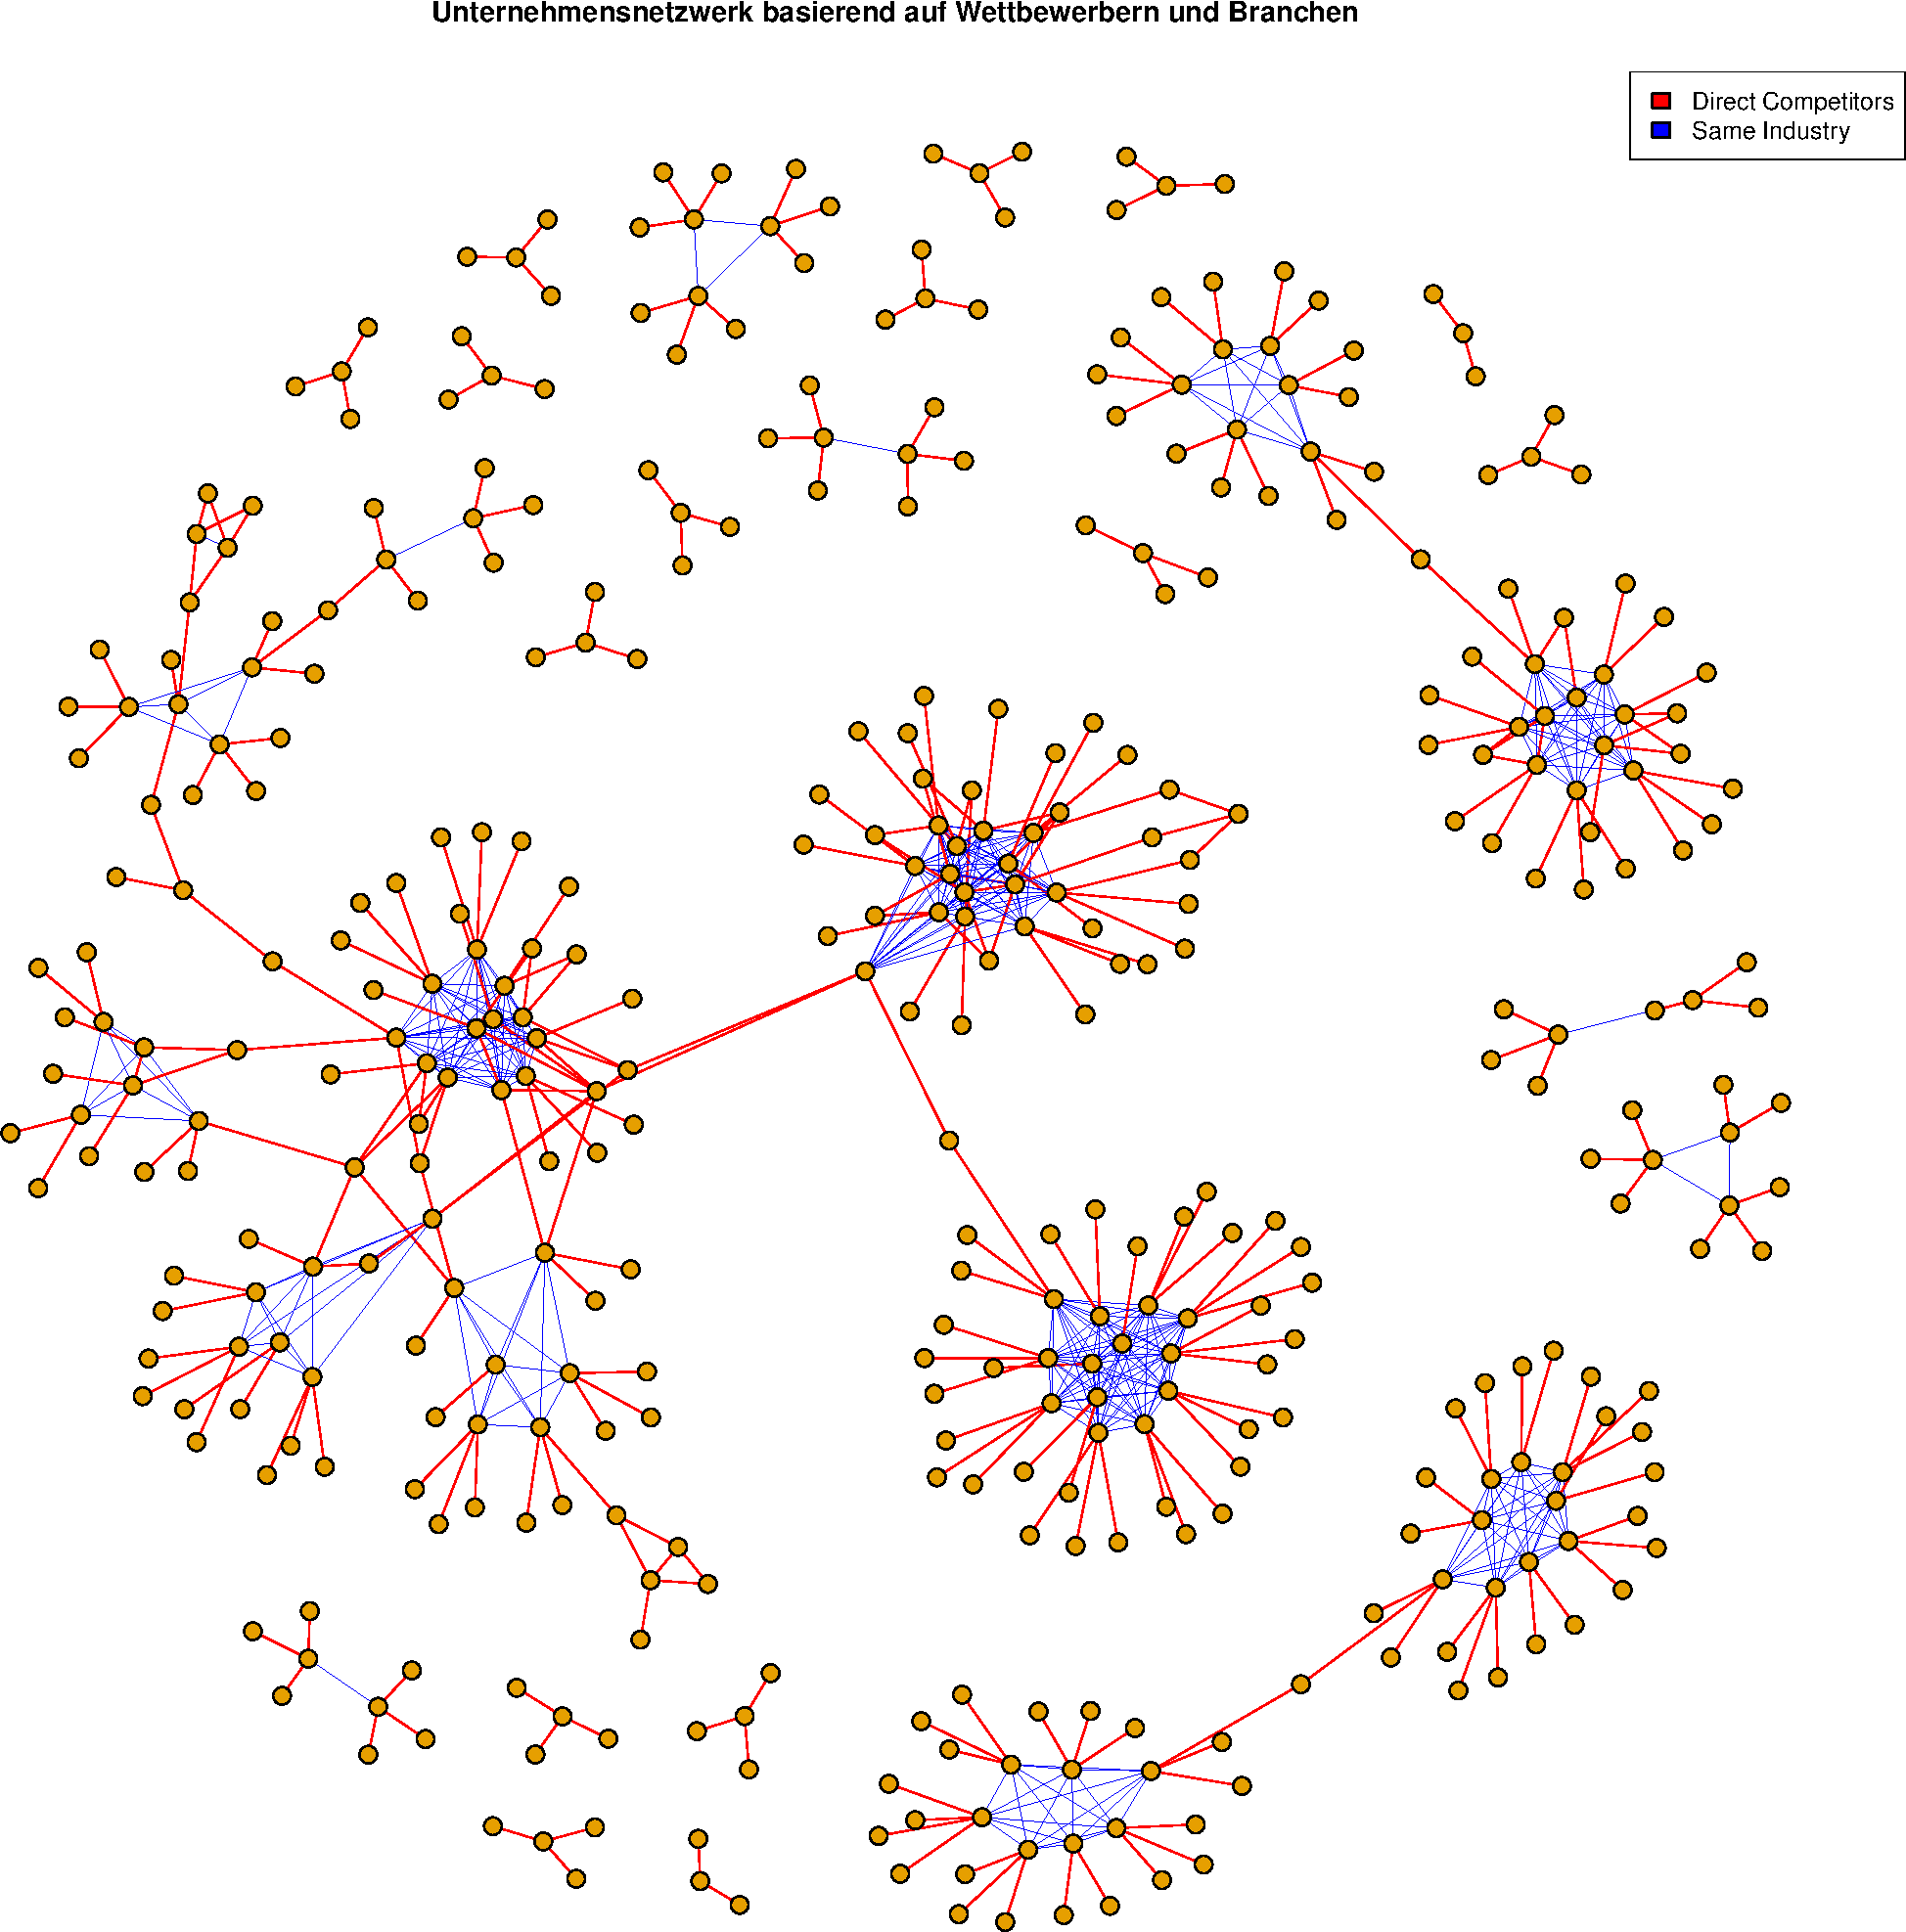
\includegraphics[keepaspectratio]{DataScience_files/figure-latex/unnamed-chunk-16-1.pdf}}

Wie zu erwarten war, sind die meisten Unternehmen Ballungszentren wie
New York, Chicago und San Francisco angesiedelt.

\subsubsection{Vergleich der Gehälter zwischen den Hotspot- und den
anderen
Regionen}\label{vergleich-der-gehuxe4lter-zwischen-den-hotspot--und-den-anderen-regionen}

\begin{Shaded}
\begin{Highlighting}[]
\CommentTok{\# Ausgabe der farbigen Standorte}
\FunctionTok{print}\NormalTok{(large\_locations)}
\end{Highlighting}
\end{Shaded}

\begin{verbatim}
## [1] "Chicago, IL"       "New York, NY"      "San Francisco, CA"
\end{verbatim}

\begin{Shaded}
\begin{Highlighting}[]
\CommentTok{\# Filterung der Daten für die Hotspot{-}Regionen}
\NormalTok{data\_hotspots }\OtherTok{\textless{}{-}}\NormalTok{ data }\SpecialCharTok{\%\textgreater{}\%}
  \FunctionTok{filter}\NormalTok{(}\StringTok{\textasciigrave{}}\AttributeTok{Location}\StringTok{\textasciigrave{}} \SpecialCharTok{\%in\%}\NormalTok{ large\_locations)}

\CommentTok{\# Filterung der Daten für die anderen Regionen}
\NormalTok{data\_other }\OtherTok{\textless{}{-}}\NormalTok{ data }\SpecialCharTok{\%\textgreater{}\%}
  \FunctionTok{filter}\NormalTok{(}\SpecialCharTok{!}\StringTok{\textasciigrave{}}\AttributeTok{Location}\StringTok{\textasciigrave{}} \SpecialCharTok{\%in\%}\NormalTok{ large\_locations)}

\CommentTok{\# Durchschnittsgehalt in den Hotspot{-}Regionen}
\NormalTok{avg\_salary\_hotspots }\OtherTok{\textless{}{-}} \FunctionTok{mean}\NormalTok{(data\_hotspots}\SpecialCharTok{$}\StringTok{\textasciigrave{}}\AttributeTok{Salary Estimate}\StringTok{\textasciigrave{}}\NormalTok{, }\AttributeTok{na.rm =} \ConstantTok{TRUE}\NormalTok{)}

\CommentTok{\# Durchschnittsgehalt in den anderen Regionen}
\NormalTok{avg\_salary\_other }\OtherTok{\textless{}{-}} \FunctionTok{mean}\NormalTok{(data\_other}\SpecialCharTok{$}\StringTok{\textasciigrave{}}\AttributeTok{Salary Estimate}\StringTok{\textasciigrave{}}\NormalTok{, }\AttributeTok{na.rm =} \ConstantTok{TRUE}\NormalTok{)}

\CommentTok{\# Erstellung eines Balkendiagramms}
\FunctionTok{ggplot}\NormalTok{(}\AttributeTok{data =} \FunctionTok{data.frame}\NormalTok{(}\AttributeTok{Region =} \FunctionTok{c}\NormalTok{(}\StringTok{"Hotspot"}\NormalTok{, }\StringTok{"Other"}\NormalTok{),}
                         \AttributeTok{Average\_Salary =} \FunctionTok{c}\NormalTok{(avg\_salary\_hotspots,}
\NormalTok{                                            avg\_salary\_other)),}
       \FunctionTok{aes}\NormalTok{(}\AttributeTok{x =}\NormalTok{ Region, }\AttributeTok{y =}\NormalTok{ Average\_Salary, }\AttributeTok{fill =}\NormalTok{ Region)) }\SpecialCharTok{+}
  \FunctionTok{geom\_bar}\NormalTok{(}\AttributeTok{stat =} \StringTok{"identity"}\NormalTok{, }\AttributeTok{width =} \FloatTok{0.4}\NormalTok{) }\SpecialCharTok{+}
  \FunctionTok{scale\_fill\_manual}\NormalTok{(}\AttributeTok{values =} \FunctionTok{c}\NormalTok{(}\StringTok{"Hotspot"} \OtherTok{=} \StringTok{"\#FF5733"}\NormalTok{, }\StringTok{"Other"} \OtherTok{=} \StringTok{"\#33C3FF"}\NormalTok{)) }\SpecialCharTok{+}
  \FunctionTok{labs}\NormalTok{(}\AttributeTok{title =} \StringTok{"Average Salary in Hotspot vs. Other Regions"}\NormalTok{,}
       \AttributeTok{x =} \StringTok{"Region"}\NormalTok{,}
       \AttributeTok{y =} \StringTok{"Average Salary"}\NormalTok{) }\SpecialCharTok{+}
  \FunctionTok{theme\_minimal}\NormalTok{() }\SpecialCharTok{+}
  \FunctionTok{theme}\NormalTok{(}
    \AttributeTok{plot.title =} \FunctionTok{element\_text}\NormalTok{(}\AttributeTok{hjust =} \FloatTok{0.5}\NormalTok{, }\AttributeTok{size =} \DecValTok{14}\NormalTok{, }\AttributeTok{face =} \StringTok{"bold"}\NormalTok{),}
    \AttributeTok{axis.title.x =} \FunctionTok{element\_text}\NormalTok{(}\AttributeTok{size =} \DecValTok{12}\NormalTok{, }\AttributeTok{face =} \StringTok{"bold"}\NormalTok{),}
    \AttributeTok{axis.title.y =} \FunctionTok{element\_text}\NormalTok{(}\AttributeTok{size =} \DecValTok{12}\NormalTok{, }\AttributeTok{face =} \StringTok{"bold"}\NormalTok{),}
    \AttributeTok{axis.text.x =} \FunctionTok{element\_text}\NormalTok{(}\AttributeTok{size =} \DecValTok{12}\NormalTok{),}
    \AttributeTok{axis.text.y =} \FunctionTok{element\_text}\NormalTok{(}\AttributeTok{size =} \DecValTok{12}\NormalTok{),}
    \AttributeTok{legend.position =} \StringTok{"none"}
\NormalTok{  ) }\SpecialCharTok{+}
  \FunctionTok{geom\_text}\NormalTok{(}\FunctionTok{aes}\NormalTok{(}\AttributeTok{label =} \FunctionTok{round}\NormalTok{(Average\_Salary, }\DecValTok{2}\NormalTok{)), }\AttributeTok{vjust =} \SpecialCharTok{{-}}\FloatTok{0.5}\NormalTok{, }\AttributeTok{size =} \DecValTok{4}\NormalTok{)}
\end{Highlighting}
\end{Shaded}

\pandocbounded{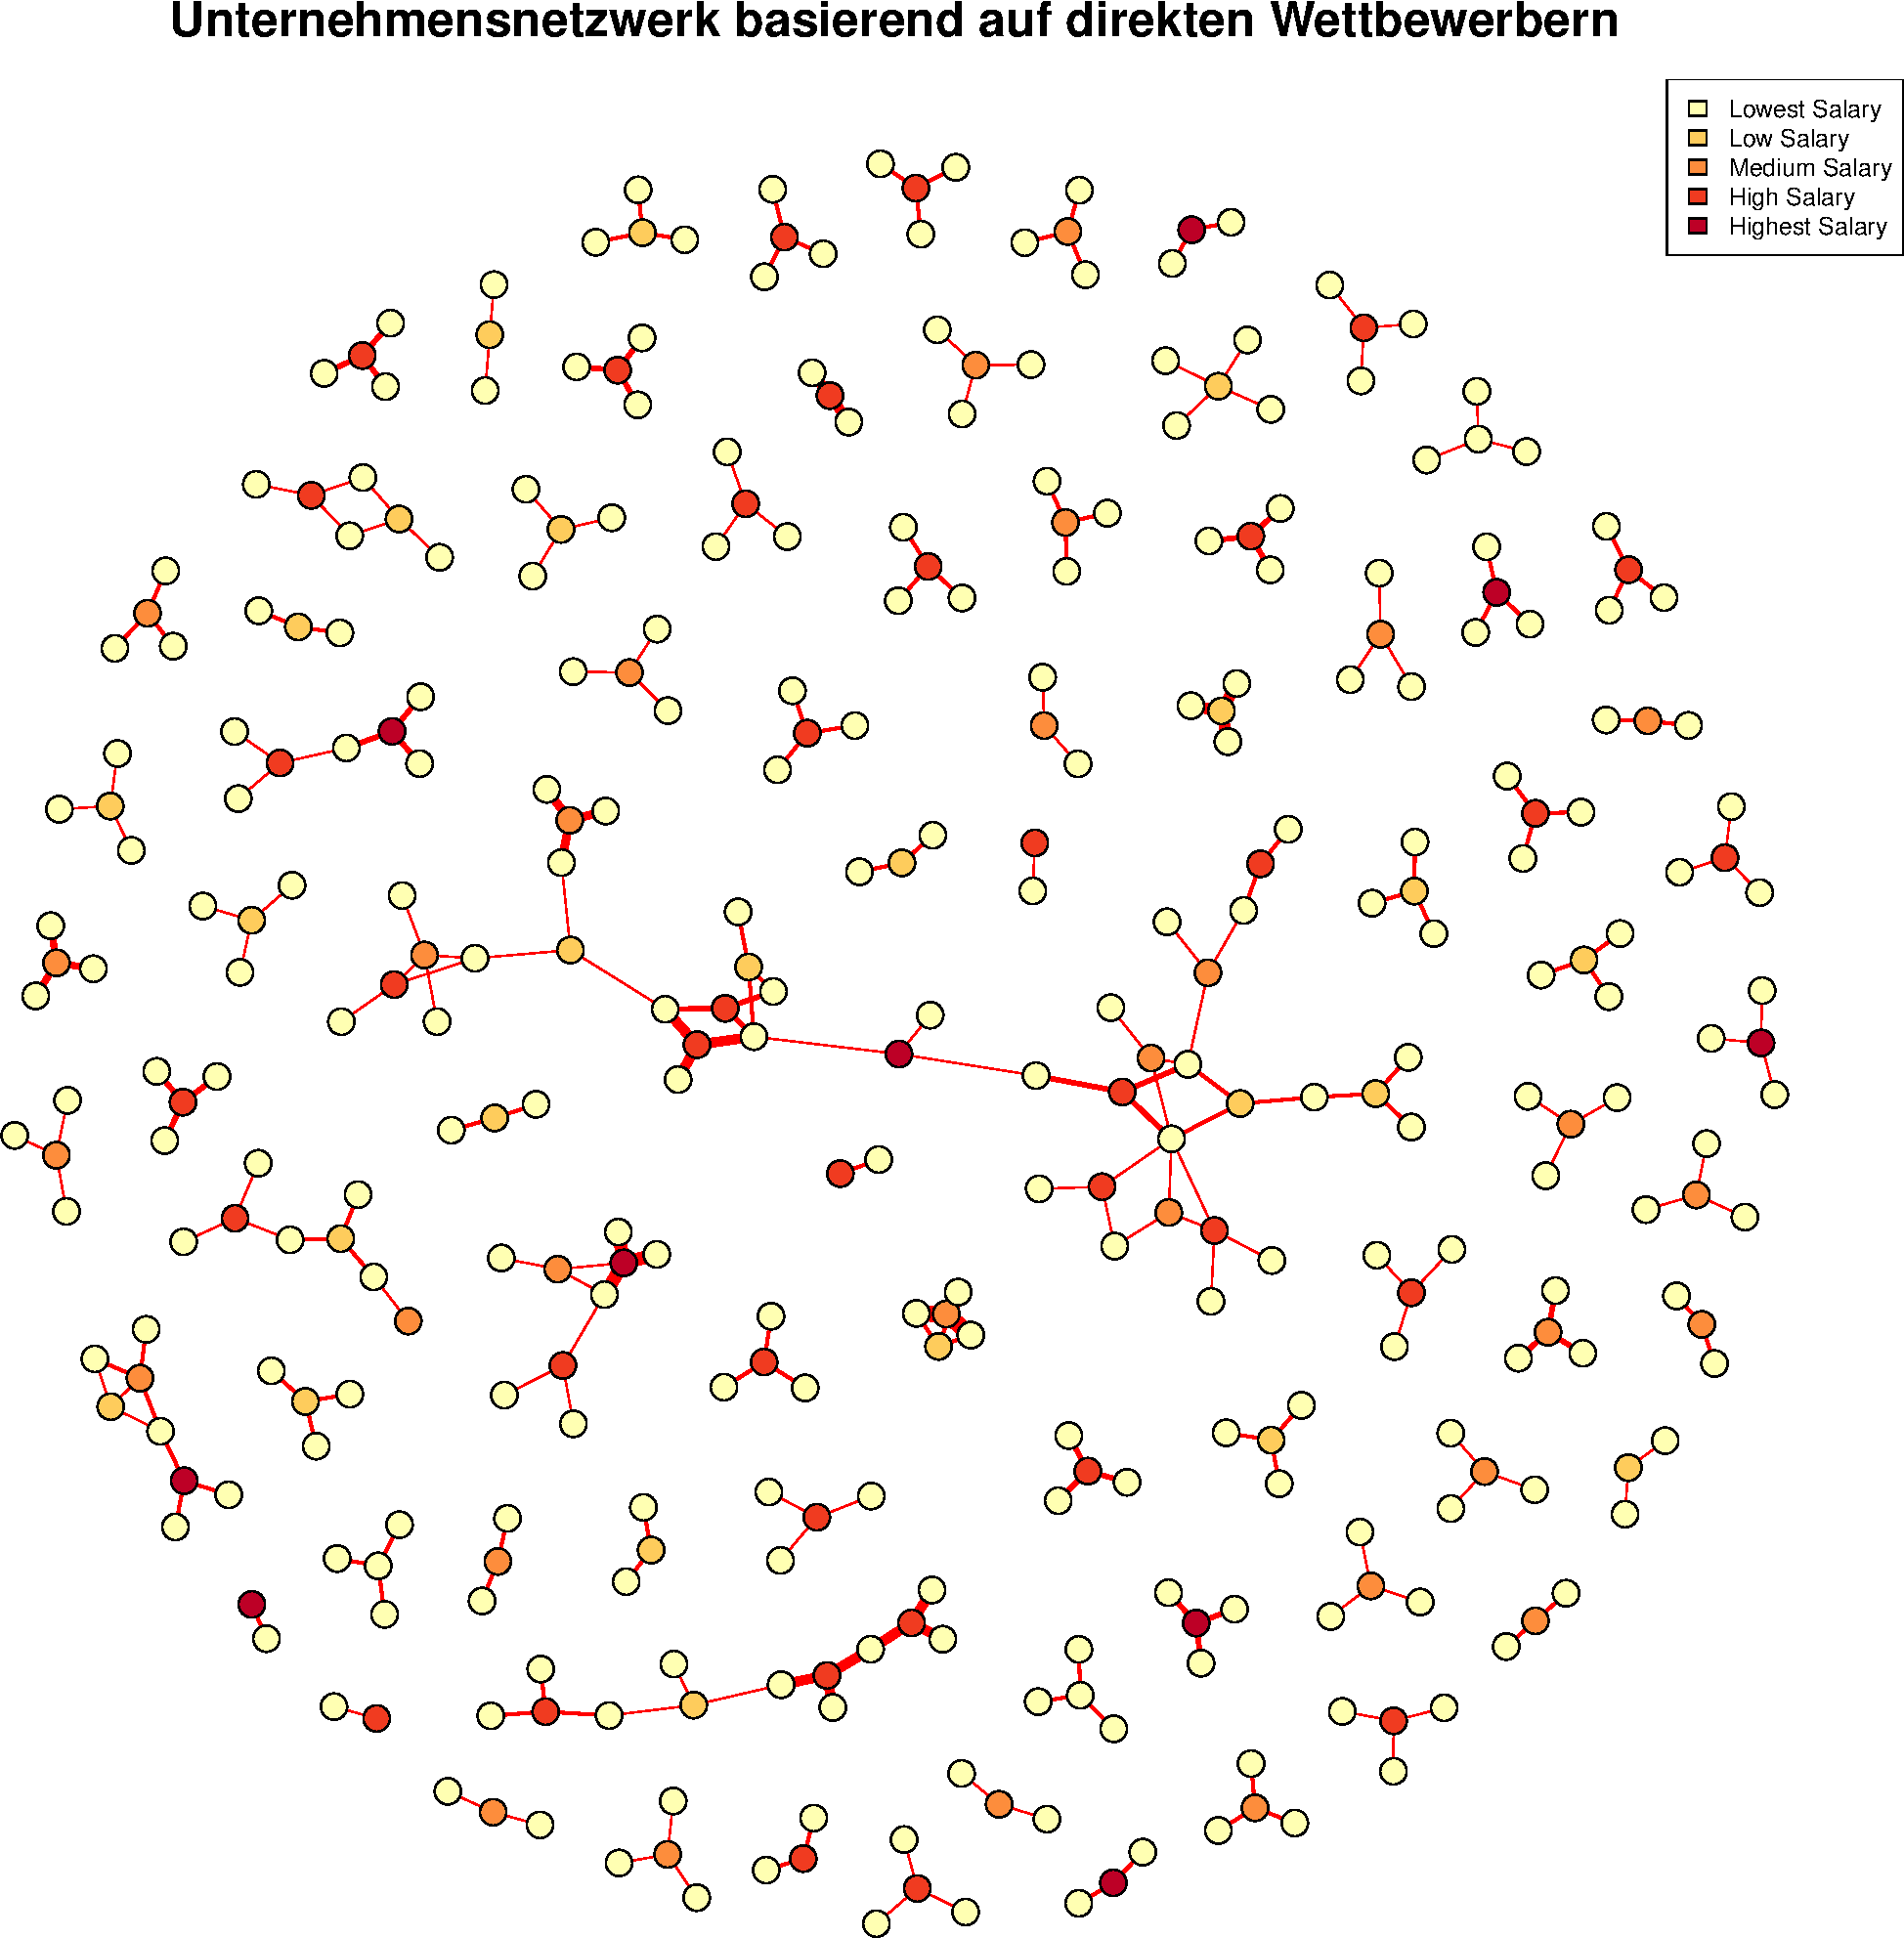
\includegraphics[keepaspectratio]{DataScience_files/figure-latex/unnamed-chunk-17-1.pdf}}

\begin{Shaded}
\begin{Highlighting}[]
\CommentTok{\# Berechnung der Gehaltsunterschiede}
\NormalTok{salary\_diff }\OtherTok{\textless{}{-}}\NormalTok{ avg\_salary\_hotspots }\SpecialCharTok{{-}}\NormalTok{ avg\_salary\_other}

\CommentTok{\# Ausgabe der Gehaltsunterschiede}
\FunctionTok{print}\NormalTok{(}\FunctionTok{paste}\NormalTok{(}\StringTok{"Durchschnittsgehalt in Hotspot{-}Regionen:"}\NormalTok{, avg\_salary\_hotspots))}
\end{Highlighting}
\end{Shaded}

\begin{verbatim}
## [1] "Durchschnittsgehalt in Hotspot-Regionen: 117.223880597015"
\end{verbatim}

\begin{Shaded}
\begin{Highlighting}[]
\FunctionTok{print}\NormalTok{(}\FunctionTok{paste}\NormalTok{(}\StringTok{"Durchschnittsgehalt in anderen Regionen:"}\NormalTok{, avg\_salary\_other))}
\end{Highlighting}
\end{Shaded}

\begin{verbatim}
## [1] "Durchschnittsgehalt in anderen Regionen: 103.59"
\end{verbatim}

\begin{Shaded}
\begin{Highlighting}[]
\FunctionTok{print}\NormalTok{(}\FunctionTok{paste}\NormalTok{(}\StringTok{"Durchschnittlicher Gehaltsunterschied:"}\NormalTok{, salary\_diff))}
\end{Highlighting}
\end{Shaded}

\begin{verbatim}
## [1] "Durchschnittlicher Gehaltsunterschied: 13.6338805970149"
\end{verbatim}

Das Ergebniss zeigt, dass entsprechend der vorher getroffenen Annahme,
die Gehälter in den Hotspot-Regionen im Durchschnitt höher sind als in
anderen Regionen. Dies impliziert eine Korrelation zwischen
geografischer Nähe und Gehaltsniveau. Eine mögliche Erlärung hierfür
könnte die höhere Lebenshaltungskosten in Ballungszentren sein, die
höhere Gehälter erforderlich machen.

Deswegen sollen am Ende dieser Arbeit die Ergebnisse der
Wettbewerbsanalyse mit den Ergebnissen der geografischen Analyse
verglichen und in Bezug gesetz werden.

\subsection{Wettbewerbsnetzwerk}\label{wettbewerbsnetzwerk}

In diesem Abschnitt wird mit der eigentlichen Analyse, dem Ziel dieser
Arbeit, der Erstellung einer Wettbewerbsanalyse begonnen.

\subsubsection{Erstellung eines
Wettbewerbsnetzwerkes}\label{erstellung-eines-wettbewerbsnetzwerkes}

Zu diesem Zweck wird ein Netzwerk erstellt, das auf den
Wettbewerbsbeziehungen zwischen Unternehmen basiert.

Die Wettbewerbsbeziehungen werden anhand der in der Spalte
``Competitors'' aufgeführten Unternehmen definiert. Die Punkte im
Netzwerk repräsentieren die Unternehmen, während die Kanten die
Wettbewerbsbeziehungen zwischen ihnen darstellen.

Die Gewichtung der Kanten erfolgt wie folgt:

\begin{itemize}
\tightlist
\item
  Direkte Wettbewerber erhalten eine Gewichtung von 1.
\item
  Unternehmen in derselben Branche, jedoch nicht als direkte
  Wettbewerber aufgeführt, erhalten eine Gewichtung von 0.5.
\end{itemize}

Branchenbezogene Wettbewerbsbeziehungen sind in blau dargestellt,
während direkte Wettbewerber in rot hervorgehoben sind.

\begin{Shaded}
\begin{Highlighting}[]
\CommentTok{\# Extrahiere Unternehmen und ihre Wettbewerber}
\NormalTok{edges }\OtherTok{\textless{}{-}}\NormalTok{ data }\SpecialCharTok{\%\textgreater{}\%}
  \FunctionTok{separate\_rows}\NormalTok{(Competitors, }\AttributeTok{sep =} \StringTok{", "}\NormalTok{) }\SpecialCharTok{\%\textgreater{}\%}
  \FunctionTok{select}\NormalTok{(}\StringTok{\textasciigrave{}}\AttributeTok{Company Name}\StringTok{\textasciigrave{}}\NormalTok{, Competitors) }\SpecialCharTok{\%\textgreater{}\%}
  \FunctionTok{rename}\NormalTok{(}\AttributeTok{from =} \StringTok{\textasciigrave{}}\AttributeTok{Company Name}\StringTok{\textasciigrave{}}\NormalTok{, }\AttributeTok{to =}\NormalTok{ Competitors) }\SpecialCharTok{\%\textgreater{}\%}
  \FunctionTok{mutate}\NormalTok{(}\AttributeTok{weight =} \DecValTok{1}\NormalTok{)  }\CommentTok{\# Gewichtung für direkte Wettbewerber}

\CommentTok{\# Füge Unternehmen in derselben Branche mit Gewichtung 0.5 hinzu}
\NormalTok{industry\_edges }\OtherTok{\textless{}{-}}\NormalTok{ data }\SpecialCharTok{\%\textgreater{}\%}
  \FunctionTok{select}\NormalTok{(}\StringTok{\textasciigrave{}}\AttributeTok{Company Name}\StringTok{\textasciigrave{}}\NormalTok{, Industry) }\SpecialCharTok{\%\textgreater{}\%}
  \FunctionTok{inner\_join}\NormalTok{(}
\NormalTok{    data }\SpecialCharTok{\%\textgreater{}\%} \FunctionTok{select}\NormalTok{(}\StringTok{\textasciigrave{}}\AttributeTok{Company Name}\StringTok{\textasciigrave{}}\NormalTok{, Industry),}
    \AttributeTok{by =} \StringTok{"Industry"}\NormalTok{,}
    \AttributeTok{relationship =} \StringTok{"many{-}to{-}many"}
\NormalTok{  ) }\SpecialCharTok{\%\textgreater{}\%}
  \FunctionTok{filter}\NormalTok{(}\StringTok{\textasciigrave{}}\AttributeTok{Company Name.x}\StringTok{\textasciigrave{}} \SpecialCharTok{!=} \StringTok{\textasciigrave{}}\AttributeTok{Company Name.y}\StringTok{\textasciigrave{}}\NormalTok{) }\SpecialCharTok{\%\textgreater{}\%}
  \FunctionTok{select}\NormalTok{(}\AttributeTok{from =} \StringTok{\textasciigrave{}}\AttributeTok{Company Name.x}\StringTok{\textasciigrave{}}\NormalTok{, }\AttributeTok{to =} \StringTok{\textasciigrave{}}\AttributeTok{Company Name.y}\StringTok{\textasciigrave{}}\NormalTok{) }\SpecialCharTok{\%\textgreater{}\%}
  \FunctionTok{mutate}\NormalTok{(}\AttributeTok{weight =} \FloatTok{0.5}\NormalTok{)  }\CommentTok{\# Gewichtung für gleiche Branche}

\CommentTok{\# Kombiniere beide Datensätze}
\NormalTok{all\_edges }\OtherTok{\textless{}{-}} \FunctionTok{bind\_rows}\NormalTok{(edges, industry\_edges)}

\CommentTok{\# Erstelle den Graphen}
\NormalTok{g\_competitors }\OtherTok{\textless{}{-}} \FunctionTok{graph\_from\_data\_frame}\NormalTok{(all\_edges, }\AttributeTok{directed =} \ConstantTok{FALSE}\NormalTok{)}

\CommentTok{\# Entferne mehrere Kanten zwischen denselben Punkten}
\NormalTok{g\_competitors }\OtherTok{\textless{}{-}} \FunctionTok{simplify}\NormalTok{(g\_competitors, }\AttributeTok{remove.multiple =} \ConstantTok{TRUE}\NormalTok{,}
                          \AttributeTok{edge.attr.comb =} \StringTok{"first"}\NormalTok{)}

\CommentTok{\# Setze die Farben der Kanten basierend auf der Gewichtung}
\FunctionTok{E}\NormalTok{(g\_competitors)}\SpecialCharTok{$}\NormalTok{color }\OtherTok{\textless{}{-}} \FunctionTok{ifelse}\NormalTok{(}\FunctionTok{E}\NormalTok{(g\_competitors)}\SpecialCharTok{$}\NormalTok{weight }\SpecialCharTok{==} \DecValTok{1}\NormalTok{, }\StringTok{"red"}\NormalTok{, }\StringTok{"blue"}\NormalTok{)}

\CommentTok{\# Visualisiere das Netzwerk mit kleineren Knoten}
\FunctionTok{plot}\NormalTok{(g\_competitors, }\AttributeTok{vertex.label =} \ConstantTok{NA}\NormalTok{,}
     \AttributeTok{vertex.size =} \DecValTok{2}\NormalTok{,  }\CommentTok{\# Kleinere Knoten}
     \AttributeTok{edge.width =} \FunctionTok{E}\NormalTok{(g\_competitors)}\SpecialCharTok{$}\NormalTok{weight,  }\CommentTok{\# Gewichtung der Kanten}
     \AttributeTok{edge.arrow.size =} \FloatTok{0.5}\NormalTok{,  }\CommentTok{\# Kleinere Pfeile}
     \AttributeTok{layout =}\NormalTok{ layout\_with\_fr)}

\FunctionTok{title}\NormalTok{(}\AttributeTok{main =} \StringTok{"Unternehmensnetzwerk basierend auf Wettbewerbern und Branchen"}\NormalTok{, }\AttributeTok{cex.main =} \DecValTok{2}\NormalTok{)}


\CommentTok{\# Legende für Kantenfarben}
\FunctionTok{legend}\NormalTok{(}\StringTok{"topright"}\NormalTok{, }\AttributeTok{legend =} \FunctionTok{c}\NormalTok{(}\StringTok{"Direct Competitors"}\NormalTok{, }\StringTok{"Same Industry"}\NormalTok{),}
       \AttributeTok{fill =} \FunctionTok{c}\NormalTok{(}\StringTok{"red"}\NormalTok{, }\StringTok{"blue"}\NormalTok{))}
\end{Highlighting}
\end{Shaded}

\pandocbounded{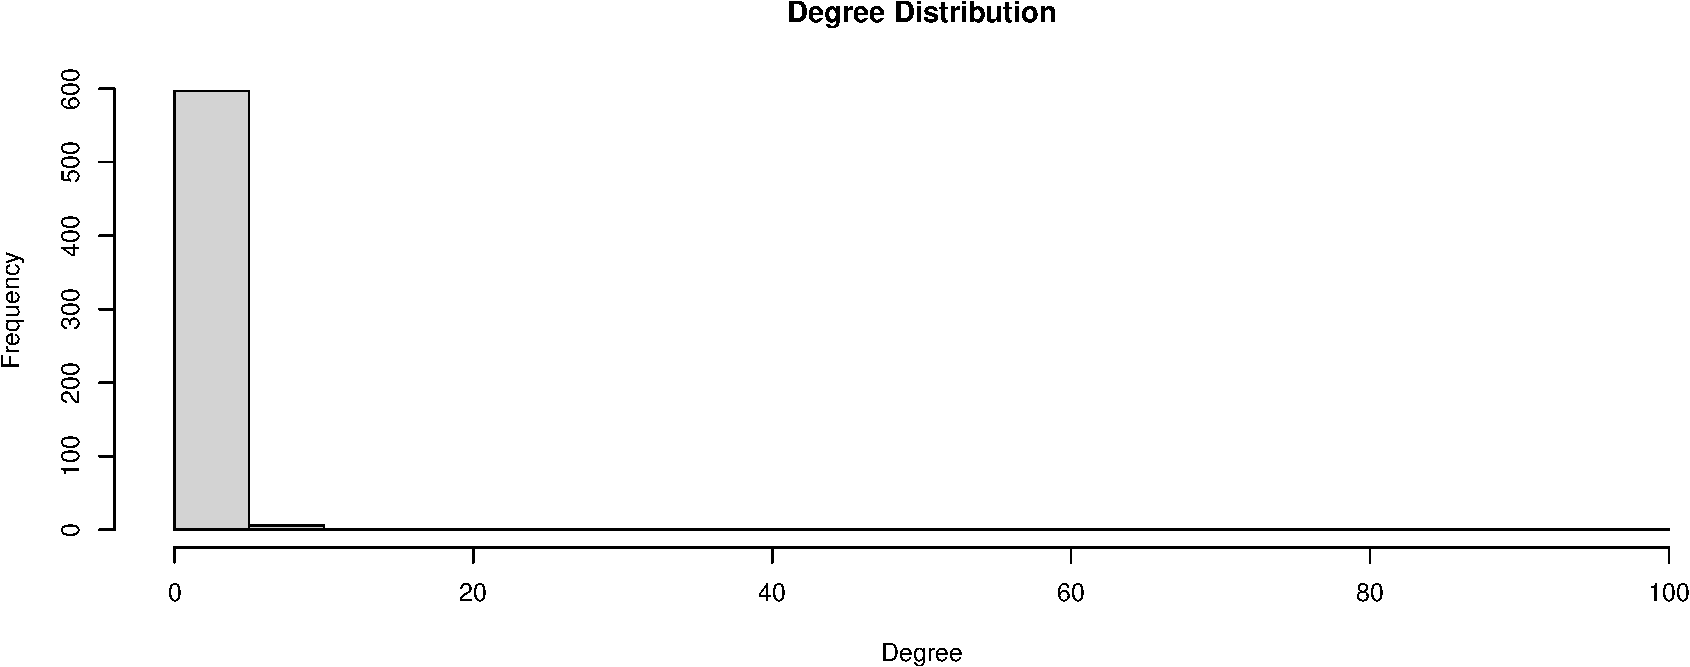
\includegraphics[keepaspectratio]{DataScience_files/figure-latex/unnamed-chunk-19-1.pdf}}
Es lassen sich einige interessante Beobachtungen aus dem Netzwerk
ziehen. Einerseits sind ganz eindeutig Branchencluster zu erkennen, die
auf die Branchenzugehörigkeit der Unternehmen hinweisen.

\begin{Shaded}
\begin{Highlighting}[]
\CommentTok{\# Ausgeben der 10 häufigsten Branchen im Netzwerk}
\NormalTok{top\_industries }\OtherTok{\textless{}{-}}\NormalTok{ data }\SpecialCharTok{\%\textgreater{}\%}
  \FunctionTok{count}\NormalTok{(Industry, }\AttributeTok{sort =} \ConstantTok{TRUE}\NormalTok{) }\SpecialCharTok{\%\textgreater{}\%}
  \FunctionTok{head}\NormalTok{(}\DecValTok{10}\NormalTok{)}

\CommentTok{\# Welche Unternehmen sind in mehreren Branchen vertreten?}
\NormalTok{multi\_industry\_companies }\OtherTok{\textless{}{-}}\NormalTok{ data }\SpecialCharTok{\%\textgreater{}\%}
  \FunctionTok{group\_by}\NormalTok{(}\StringTok{\textasciigrave{}}\AttributeTok{Company Name}\StringTok{\textasciigrave{}}\NormalTok{) }\SpecialCharTok{\%\textgreater{}\%}
  \FunctionTok{summarise}\NormalTok{(}\AttributeTok{Num\_Industries =} \FunctionTok{n\_distinct}\NormalTok{(Industry)) }\SpecialCharTok{\%\textgreater{}\%}
  \FunctionTok{filter}\NormalTok{(Num\_Industries }\SpecialCharTok{\textgreater{}} \DecValTok{1}\NormalTok{) }\SpecialCharTok{\%\textgreater{}\%}
  \FunctionTok{arrange}\NormalTok{(}\FunctionTok{desc}\NormalTok{(Num\_Industries))}

\CommentTok{\# Sind Unternehmen enthalten, die in mehreren Branchen vertreten sind?}
\ControlFlowTok{if}\NormalTok{ (}\FunctionTok{nrow}\NormalTok{(multi\_industry\_companies) }\SpecialCharTok{==} \DecValTok{0}\NormalTok{) \{}
  \FunctionTok{print}\NormalTok{(}\StringTok{"Keine Unternehmen in mehreren Branchen vertreten."}\NormalTok{)}
\NormalTok{\} }\ControlFlowTok{else}\NormalTok{ \{}
  \FunctionTok{print}\NormalTok{(}\StringTok{"Unternehmen in mehreren Branchen vertreten."}\NormalTok{)}
\NormalTok{\}}
\end{Highlighting}
\end{Shaded}

\begin{verbatim}
## [1] "Keine Unternehmen in mehreren Branchen vertreten."
\end{verbatim}

Jedoch sind keine Unternehmen in mehreren Branchen vertreten, was darauf
hindeutet, dass die Branchenzugehörigkeit eindeutig ist. Aber es gibt
einige Unternehmen, die mit direkter Konkurrenz die verschiedenen
Branchen verbinden. Dies könnte auf eine Diversifikation der
Geschäftsfelder hindeuten, die eine breitere Wettbewerbsbasis schafft.

Da aber wie oberhalb dargestellt, die Branchenzugehörigkeit eindeutig
ist, und somit die Branchenzugehörigkeit keinen Mehrwert für die Analyse
bietet, wird diese nicht weiter verfolgt.

\subsubsection{Betrachtung fokussiert auf direkte
Wettbewerber}\label{betrachtung-fokussiert-auf-direkte-wettbewerber}

Aus diesem Grund wird das Netzwerk auf direkte Wettbewerber beschränkt,
um die Analyse zu vereinfachen und die Relevanz der
Wettbewerbsbeziehungen zu erhöhen.

\begin{Shaded}
\begin{Highlighting}[]
\CommentTok{\# Extrahiere Unternehmen und ihre Wettbewerber}
\NormalTok{edges }\OtherTok{\textless{}{-}}\NormalTok{ data }\SpecialCharTok{\%\textgreater{}\%}
  \FunctionTok{separate\_rows}\NormalTok{(Competitors, }\AttributeTok{sep =} \StringTok{", "}\NormalTok{) }\SpecialCharTok{\%\textgreater{}\%}
  \FunctionTok{select}\NormalTok{(}\StringTok{\textasciigrave{}}\AttributeTok{Company Name}\StringTok{\textasciigrave{}}\NormalTok{, Competitors) }\SpecialCharTok{\%\textgreater{}\%}
  \FunctionTok{rename}\NormalTok{(}\AttributeTok{from =} \StringTok{\textasciigrave{}}\AttributeTok{Company Name}\StringTok{\textasciigrave{}}\NormalTok{, }\AttributeTok{to =}\NormalTok{ Competitors) }\SpecialCharTok{\%\textgreater{}\%}
  \FunctionTok{mutate}\NormalTok{(}\AttributeTok{weight =} \DecValTok{1}\NormalTok{)  }\CommentTok{\# Gewichtung für direkte Wettbewerber}

\CommentTok{\# Summiere die Gewichtungen für mehrere Kanten zwischen denselben Punkten}
\NormalTok{edge\_weights }\OtherTok{\textless{}{-}}\NormalTok{ edges }\SpecialCharTok{\%\textgreater{}\%}
  \FunctionTok{group\_by}\NormalTok{(from, to) }\SpecialCharTok{\%\textgreater{}\%}
  \FunctionTok{summarise}\NormalTok{(}\AttributeTok{weight =} \FunctionTok{sum}\NormalTok{(weight), }\AttributeTok{.groups =} \StringTok{\textquotesingle{}drop\textquotesingle{}}\NormalTok{)}

\CommentTok{\# Erstelle den Graphen nur mit direkten Wettbewerbern}
\NormalTok{g\_direct\_competitors }\OtherTok{\textless{}{-}} \FunctionTok{graph\_from\_data\_frame}\NormalTok{(edge\_weights, }\AttributeTok{directed =} \ConstantTok{FALSE}\NormalTok{)}

\CommentTok{\# Setze die Gewichtungen der Kanten im Graphen}
\FunctionTok{E}\NormalTok{(g\_direct\_competitors)}\SpecialCharTok{$}\NormalTok{weight }\OtherTok{\textless{}{-}}\NormalTok{ edge\_weights}\SpecialCharTok{$}\NormalTok{weight}

\CommentTok{\# Füge die Gehaltsdaten hinzu und berechne das durchschnittliche Gehalt pro Unternehmen}
\NormalTok{salary\_data }\OtherTok{\textless{}{-}}\NormalTok{ data }\SpecialCharTok{\%\textgreater{}\%}
  \FunctionTok{group\_by}\NormalTok{(}\StringTok{\textasciigrave{}}\AttributeTok{Company Name}\StringTok{\textasciigrave{}}\NormalTok{) }\SpecialCharTok{\%\textgreater{}\%}
  \FunctionTok{summarise}\NormalTok{(}\AttributeTok{AverageSalary =} \FunctionTok{mean}\NormalTok{(}\StringTok{\textasciigrave{}}\AttributeTok{Salary Estimate}\StringTok{\textasciigrave{}}\NormalTok{, }\AttributeTok{na.rm =} \ConstantTok{TRUE}\NormalTok{))}

\CommentTok{\# Füge die Gehaltsdaten zu den Knoten des Graphen hinzu}
\FunctionTok{V}\NormalTok{(g\_direct\_competitors)}\SpecialCharTok{$}\NormalTok{salary }\OtherTok{\textless{}{-}}\NormalTok{ salary\_data}\SpecialCharTok{$}\NormalTok{AverageSalary[}\FunctionTok{match}\NormalTok{(}\FunctionTok{V}\NormalTok{(g\_direct\_competitors)}\SpecialCharTok{$}\NormalTok{name, salary\_data}\SpecialCharTok{$}\StringTok{\textasciigrave{}}\AttributeTok{Company Name}\StringTok{\textasciigrave{}}\NormalTok{)]}

\CommentTok{\# Setze die Farben der Knoten basierend auf den Gehältern}
\NormalTok{salary\_quantiles }\OtherTok{\textless{}{-}} \FunctionTok{quantile}\NormalTok{(}\FunctionTok{V}\NormalTok{(g\_direct\_competitors)}\SpecialCharTok{$}\NormalTok{salary, }\AttributeTok{probs =} \FunctionTok{seq}\NormalTok{(}\DecValTok{0}\NormalTok{, }\DecValTok{1}\NormalTok{, }\AttributeTok{length.out =} \DecValTok{6}\NormalTok{), }\AttributeTok{na.rm =} \ConstantTok{TRUE}\NormalTok{)}
\NormalTok{color\_palette }\OtherTok{\textless{}{-}} \FunctionTok{brewer.pal}\NormalTok{(}\DecValTok{5}\NormalTok{, }\StringTok{"YlOrRd"}\NormalTok{)}
\FunctionTok{V}\NormalTok{(g\_direct\_competitors)}\SpecialCharTok{$}\NormalTok{color }\OtherTok{\textless{}{-}} \FunctionTok{cut}\NormalTok{(}\FunctionTok{V}\NormalTok{(g\_direct\_competitors)}\SpecialCharTok{$}\NormalTok{salary, }
                                     \AttributeTok{breaks =}\NormalTok{ salary\_quantiles, }
                                     \AttributeTok{labels =} \ConstantTok{FALSE}\NormalTok{, }
                                     \AttributeTok{include.lowest =} \ConstantTok{TRUE}\NormalTok{)}
\FunctionTok{V}\NormalTok{(g\_direct\_competitors)}\SpecialCharTok{$}\NormalTok{color }\OtherTok{\textless{}{-}}\NormalTok{ color\_palette[}\FunctionTok{V}\NormalTok{(g\_direct\_competitors)}\SpecialCharTok{$}\NormalTok{color]}

\CommentTok{\# Setze die Farben der Kanten basierend auf der Gewichtung}
\FunctionTok{E}\NormalTok{(g\_direct\_competitors)}\SpecialCharTok{$}\NormalTok{color }\OtherTok{\textless{}{-}} \StringTok{"red"}

\CommentTok{\# Visualisiere das Netzwerk mit kleineren Knoten}
\FunctionTok{plot}\NormalTok{(g\_direct\_competitors, }\AttributeTok{vertex.label =} \ConstantTok{NA}\NormalTok{,}
     \AttributeTok{vertex.size =} \DecValTok{3}\NormalTok{,  }\CommentTok{\# Kleinere Knoten}
     \AttributeTok{edge.width =} \DecValTok{1} \SpecialCharTok{*} \FunctionTok{E}\NormalTok{(g\_direct\_competitors)}\SpecialCharTok{$}\NormalTok{weight,  }\CommentTok{\# Reduzierte Gewichtung der Kanten}
     \AttributeTok{edge.arrow.size =} \DecValTok{1}\NormalTok{,}
     \AttributeTok{layout =}\NormalTok{ layout\_with\_fr}
\NormalTok{)}
\FunctionTok{title}\NormalTok{(}\AttributeTok{main =} \StringTok{"Unternehmensnetzwerk basierend auf direkten Wettbewerbern"}\NormalTok{, }\AttributeTok{cex.main =} \DecValTok{2}\NormalTok{)}


\CommentTok{\# Legende für Knotenfarben}
\FunctionTok{legend}\NormalTok{(}\StringTok{"topright"}\NormalTok{, }\AttributeTok{legend =} \FunctionTok{c}\NormalTok{(}\StringTok{"Lowest Salary"}\NormalTok{, }\StringTok{"Low Salary"}\NormalTok{, }\StringTok{"Medium Salary"}\NormalTok{, }\StringTok{"High Salary"}\NormalTok{, }\StringTok{"Highest Salary"}\NormalTok{),}
       \AttributeTok{fill =}\NormalTok{ color\_palette)}
\end{Highlighting}
\end{Shaded}

\pandocbounded{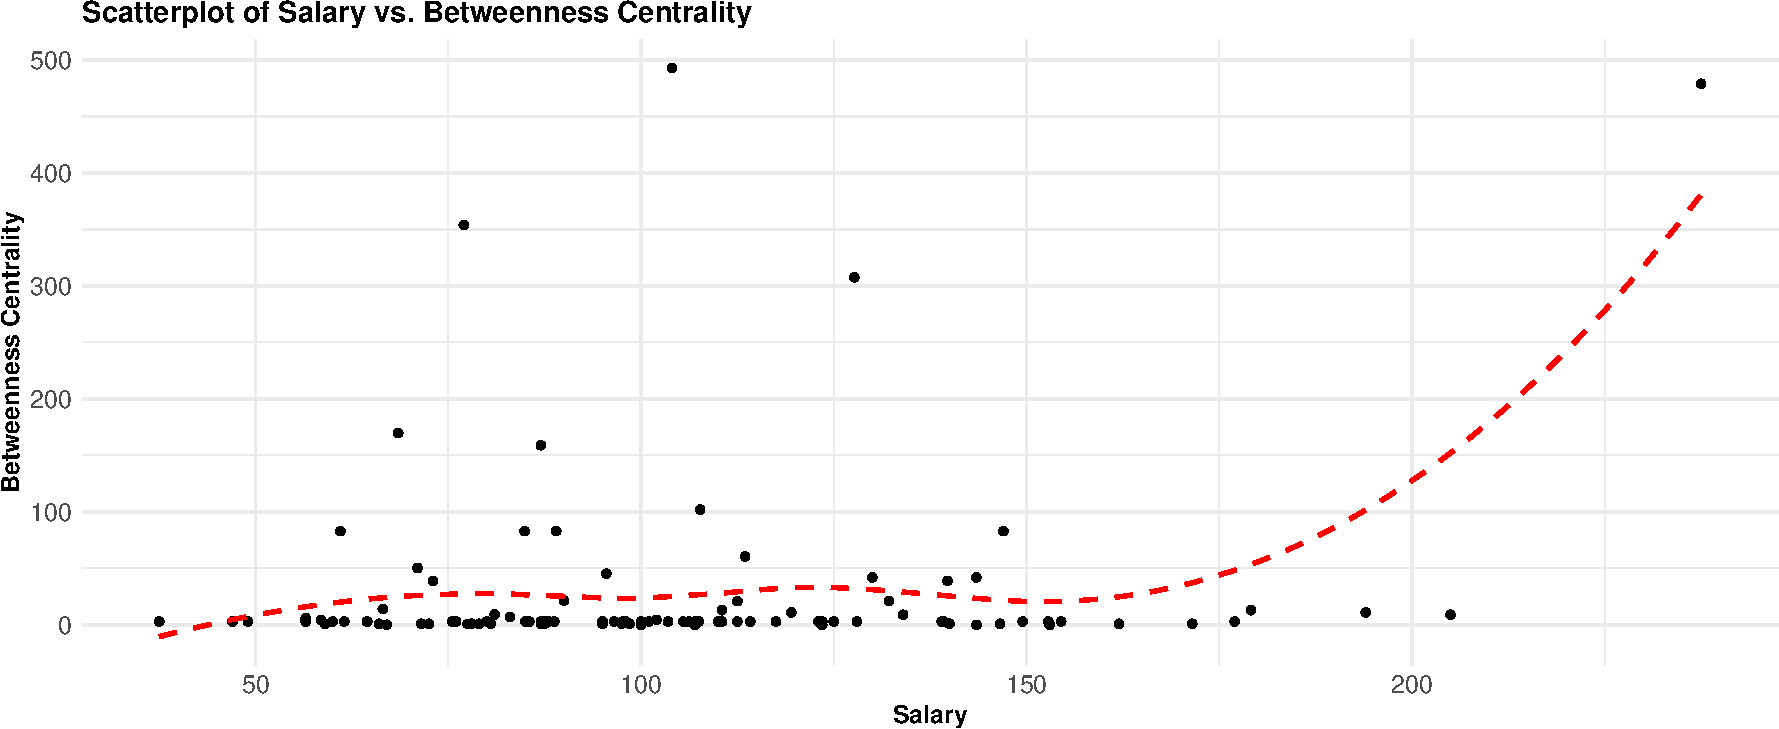
\includegraphics[keepaspectratio]{DataScience_files/figure-latex/unnamed-chunk-21-1.pdf}}

\begin{Shaded}
\begin{Highlighting}[]
\CommentTok{\# Ausgabe der Gehälter der Unternehmen}
\NormalTok{salary\_data }\OtherTok{\textless{}{-}}\NormalTok{ data }\SpecialCharTok{\%\textgreater{}\%}
  \FunctionTok{group\_by}\NormalTok{(}\StringTok{\textasciigrave{}}\AttributeTok{Company Name}\StringTok{\textasciigrave{}}\NormalTok{) }\SpecialCharTok{\%\textgreater{}\%}
  \FunctionTok{summarise}\NormalTok{(}\AttributeTok{AverageSalary =} \FunctionTok{mean}\NormalTok{(}\StringTok{\textasciigrave{}}\AttributeTok{Salary Estimate}\StringTok{\textasciigrave{}}\NormalTok{, }\AttributeTok{na.rm =} \ConstantTok{TRUE}\NormalTok{)) }\SpecialCharTok{\%\textgreater{}\%}
  \FunctionTok{arrange}\NormalTok{(}\FunctionTok{desc}\NormalTok{(AverageSalary))}

\CommentTok{\# Ausgabe aller Unternehmen zusammen mit ihren Gehältern}
\FunctionTok{print}\NormalTok{(salary\_data, }\AttributeTok{n =} \DecValTok{10}\NormalTok{)}
\end{Highlighting}
\end{Shaded}

\begin{verbatim}
## # A tibble: 107 x 2
##    `Company Name`           AverageSalary
##    <chr>                            <dbl>
##  1 Gallup                            238.
##  2 Credit Sesame                     205 
##  3 The Climate Corporation           194 
##  4 Liberty Mutual Insurance          179.
##  5 Samsung Research America          177 
##  6 Western Digital                   172.
##  7 Glassdoor                         162 
##  8 Netskope                          154.
##  9 Factual                           153 
## 10 Visa Inc.                         153.
## # i 97 more rows
\end{verbatim}

Kommentar!!!\ldots..

TODO

\subsection{Zentralitätsanalyse innerhalb des
Netzwerkes}\label{zentralituxe4tsanalyse-innerhalb-des-netzwerkes}

Die hier präsentierten Zentralitätsmaße lassen sich unmittelbar auf die
Gehaltsstrukturen im Kontext des Wettbewerbsnetzwerks anwenden. Auf
diese Weise könnten sie dazu beitragen, die Position eines Unternehmens
in Bezug auf seine Wettbewerber hinsichtlich der Gehälter zu bestimmen.

Folgend wird die Berechnung der Zentralitätsmaße für die Unternehmen im
Wettbewerbsnetzwerk dargelegt.

\begin{Shaded}
\begin{Highlighting}[]
\CommentTok{\# Datenauswahl für die Zentralitätsanalyse}
\NormalTok{selected\_data }\OtherTok{\textless{}{-}}\NormalTok{ data }\SpecialCharTok{\%\textgreater{}\%}
  \FunctionTok{select}\NormalTok{(}\StringTok{\textasciigrave{}}\AttributeTok{Company Name}\StringTok{\textasciigrave{}}\NormalTok{, Competitors, }\StringTok{\textasciigrave{}}\AttributeTok{Salary Estimate}\StringTok{\textasciigrave{}}\NormalTok{)}

\CommentTok{\# Extrahiere Unternehmen und ihre Wettbewerber}
\NormalTok{edges }\OtherTok{\textless{}{-}}\NormalTok{ selected\_data }\SpecialCharTok{\%\textgreater{}\%}
  \FunctionTok{separate\_rows}\NormalTok{(Competitors, }\AttributeTok{sep =} \StringTok{", "}\NormalTok{) }\SpecialCharTok{\%\textgreater{}\%}
  \FunctionTok{select}\NormalTok{(}\StringTok{\textasciigrave{}}\AttributeTok{Company Name}\StringTok{\textasciigrave{}}\NormalTok{, Competitors) }\SpecialCharTok{\%\textgreater{}\%}
  \FunctionTok{rename}\NormalTok{(}\AttributeTok{from =} \StringTok{\textasciigrave{}}\AttributeTok{Company Name}\StringTok{\textasciigrave{}}\NormalTok{, }\AttributeTok{to =}\NormalTok{ Competitors)}

\CommentTok{\# Erstelle den Graphen}
\NormalTok{g\_competitors\_zentralität }\OtherTok{\textless{}{-}} \FunctionTok{graph\_from\_data\_frame}\NormalTok{(edges, }\AttributeTok{directed =} \ConstantTok{FALSE}\NormalTok{)}


\CommentTok{\# Berechne die Zentralitätsmaße für die Knoten}
\NormalTok{degree\_centrality }\OtherTok{\textless{}{-}} \FunctionTok{degree}\NormalTok{(g\_competitors\_zentralität, }\AttributeTok{mode =} \StringTok{"all"}\NormalTok{)}
\NormalTok{betweenness\_centrality }\OtherTok{\textless{}{-}} \FunctionTok{betweenness}\NormalTok{(g\_competitors\_zentralität, }\AttributeTok{directed =} \ConstantTok{FALSE}\NormalTok{)}
\NormalTok{eigenvector\_centrality }\OtherTok{\textless{}{-}} \FunctionTok{evcent}\NormalTok{(g\_competitors\_zentralität, }\AttributeTok{directed =} \ConstantTok{FALSE}\NormalTok{)}
\end{Highlighting}
\end{Shaded}

\begin{verbatim}
## Warning: `evcent()` was deprecated in igraph 2.0.0.
## i Please use `eigen_centrality()` instead.
## This warning is displayed once every 8 hours.
## Call `lifecycle::last_lifecycle_warnings()` to see where this warning was
## generated.
\end{verbatim}

\subsubsection{Betweenness-Zentralität}\label{betweenness-zentralituxe4t}

Jetzt soll das igraph-Paket in R verwendet werden, um die
Betweenness-Zentralität für jeden Knoten zu berechnen. Unternehmen mit
hoher Betweenness-Centralität könnten strategische Wettbewerbsvorteile
aufweisen, da sie als Vermittler zwischen mehreren Konkurrenten
fungieren und dadurch den Informationsfluss beeinflussen können.

Die Unternehmen könnten höhere Gehälter anbieten, um hochqualifizierte
Arbeitskräfte zu gewinnen, die dazu beitragen, ihre zentrale Position
und die damit verbundenen Wettbewerbsvorteile zu erhalten. Alternativ
könnte ein hohes Gehalt auch als Indikator für eine hohe Nachfrage nach
qualifizierten Mitarbeitenden in solchen Schlüsselpositionen dienen, da
das Unternehmen sich in einem Bereich positioniert, der viele
strategische Informationen benötigt.

\begin{Shaded}
\begin{Highlighting}[]
\CommentTok{\# Berechne die Betweenness{-}Centrality und sortiere sie absteigend}
\NormalTok{top\_betweenness }\OtherTok{\textless{}{-}} \FunctionTok{head}\NormalTok{(}\FunctionTok{sort}\NormalTok{(betweenness\_centrality, }\AttributeTok{decreasing =} \ConstantTok{TRUE}\NormalTok{), }\DecValTok{5}\NormalTok{)}

\CommentTok{\# Erstelle ein DataFrame mit den Namen der Unternehmen und ihrer Betweenness{-}Centrality}
\NormalTok{top\_betweenness\_df }\OtherTok{\textless{}{-}} \FunctionTok{data.frame}\NormalTok{(}
  \AttributeTok{Company =} \FunctionTok{names}\NormalTok{(top\_betweenness),}
  \AttributeTok{Betweenness =} \FunctionTok{as.numeric}\NormalTok{(top\_betweenness),}
  \AttributeTok{stringsAsFactors =} \ConstantTok{FALSE}
\NormalTok{)}

\CommentTok{\# Erstellen einer Tabelle}
\FunctionTok{kable}\NormalTok{(top\_betweenness\_df, }\AttributeTok{format =} \StringTok{"latex"}\NormalTok{, }\AttributeTok{booktabs =} \ConstantTok{TRUE}\NormalTok{, }\AttributeTok{align =} \StringTok{"l"}\NormalTok{) }\SpecialCharTok{\%\textgreater{}\%}
\FunctionTok{kable\_styling}\NormalTok{(}\AttributeTok{latex\_options =} \FunctionTok{c}\NormalTok{(}\StringTok{"striped"}\NormalTok{, }\StringTok{"hold\_position"}\NormalTok{), }\AttributeTok{position =} \StringTok{"left"}\NormalTok{)}
\end{Highlighting}
\end{Shaded}

\begin{tabular}{ll}
\toprule
Company & Betweenness\\
\midrule
\cellcolor{gray!10}{PA Consulting} & \cellcolor{gray!10}{492.8571}\\
Gallup & 479.0000\\
\cellcolor{gray!10}{Booz Allen Hamilton} & \cellcolor{gray!10}{477.1818}\\
McKinsey \& Company & 462.0000\\
\cellcolor{gray!10}{General Dynamics Information Technology} & \cellcolor{gray!10}{354.0000}\\
\bottomrule
\end{tabular}

\begin{Shaded}
\begin{Highlighting}[]
\CommentTok{\# Zusammenhang zwischen durchschnittliches Gehalt und Betweenness{-}Zentralität}
\NormalTok{salary\_betweenness }\OtherTok{\textless{}{-}} \FunctionTok{data.frame}\NormalTok{(}
  \AttributeTok{Salary =}\NormalTok{ salary\_data}\SpecialCharTok{$}\NormalTok{AverageSalary,}
  \AttributeTok{Betweenness =}\NormalTok{ betweenness\_centrality[}\FunctionTok{match}\NormalTok{(salary\_data}\SpecialCharTok{$}\StringTok{\textasciigrave{}}\AttributeTok{Company Name}\StringTok{\textasciigrave{}}\NormalTok{, }\FunctionTok{names}\NormalTok{(betweenness\_centrality))]}
\NormalTok{)}

\CommentTok{\# Scatterplot mit roter, gestrichelter Trendlinie}
\FunctionTok{ggplot}\NormalTok{(salary\_betweenness, }\FunctionTok{aes}\NormalTok{(}\AttributeTok{x =}\NormalTok{ Salary, }\AttributeTok{y =}\NormalTok{ Betweenness)) }\SpecialCharTok{+}
  \FunctionTok{geom\_point}\NormalTok{() }\SpecialCharTok{+}
  \FunctionTok{geom\_smooth}\NormalTok{(}\AttributeTok{method =} \StringTok{"loess"}\NormalTok{, }\AttributeTok{se =} \ConstantTok{FALSE}\NormalTok{, }\AttributeTok{color =} \StringTok{"red"}\NormalTok{, }\AttributeTok{linetype =} \StringTok{"dashed"}\NormalTok{) }\SpecialCharTok{+}
  \FunctionTok{labs}\NormalTok{(}\AttributeTok{title =} \StringTok{"Scatterplot of Salary vs. Betweenness Centrality"}\NormalTok{,}
       \AttributeTok{x =} \StringTok{"Salary"}\NormalTok{, }\AttributeTok{y =} \StringTok{"Betweenness Centrality"}\NormalTok{) }\SpecialCharTok{+}
  \FunctionTok{theme\_minimal}\NormalTok{() }\SpecialCharTok{+}
  \FunctionTok{theme}\NormalTok{(}
    \AttributeTok{plot.title =} \FunctionTok{element\_text}\NormalTok{(}\AttributeTok{size =} \DecValTok{14}\NormalTok{, }\AttributeTok{face =} \StringTok{"bold"}\NormalTok{),}
    \AttributeTok{axis.title =} \FunctionTok{element\_text}\NormalTok{(}\AttributeTok{size =} \DecValTok{12}\NormalTok{, }\AttributeTok{face =} \StringTok{"bold"}\NormalTok{),}
    \AttributeTok{axis.text =} \FunctionTok{element\_text}\NormalTok{(}\AttributeTok{size =} \DecValTok{12}\NormalTok{)}
\NormalTok{  )}
\end{Highlighting}
\end{Shaded}

\begin{verbatim}
## `geom_smooth()` using formula = 'y ~ x'
\end{verbatim}

\pandocbounded{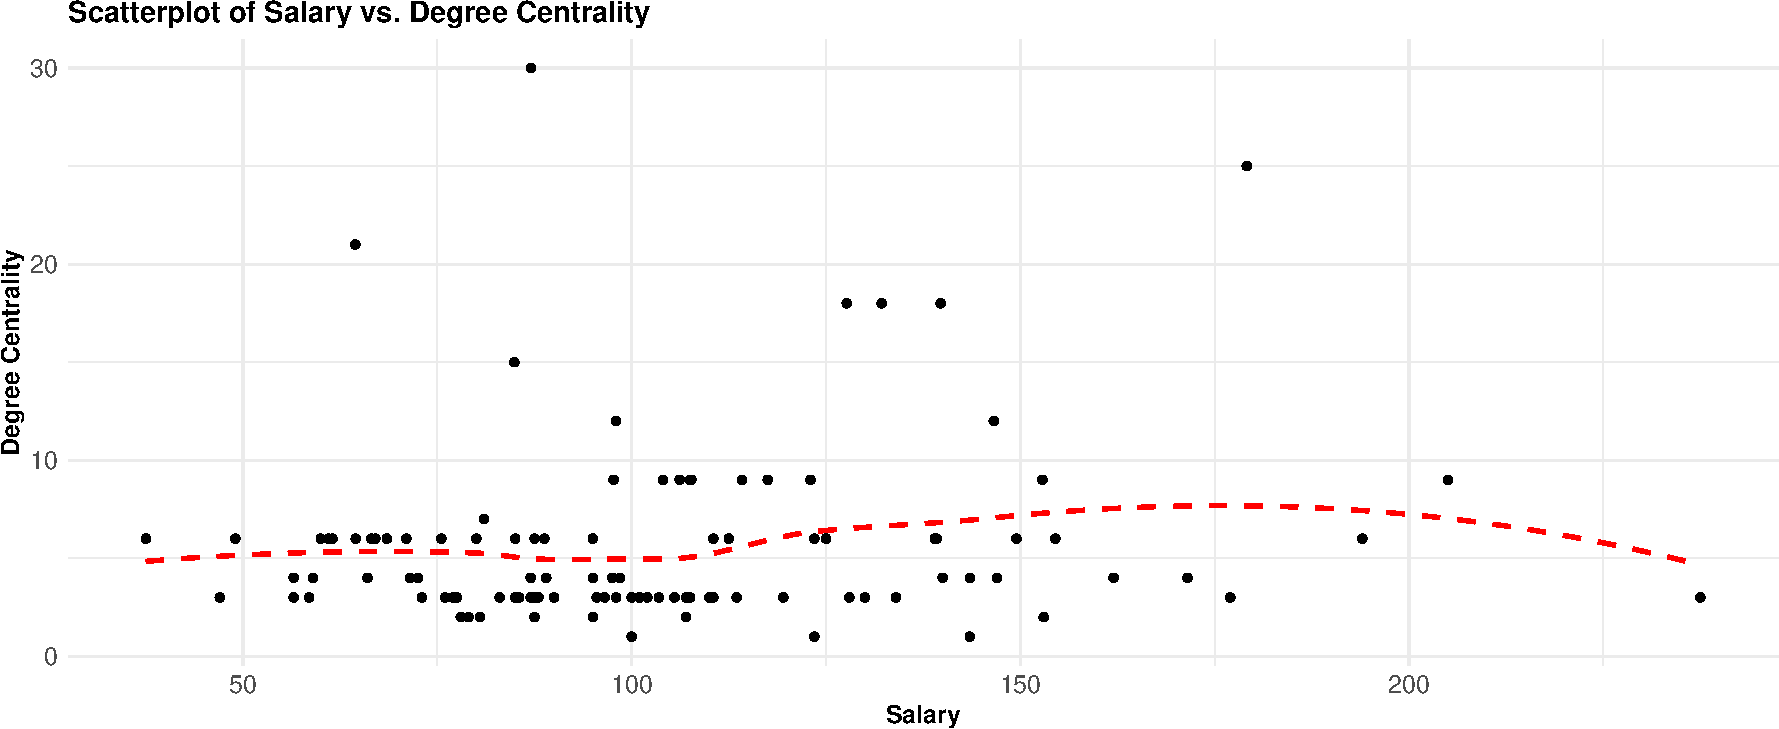
\includegraphics[keepaspectratio]{DataScience_files/figure-latex/unnamed-chunk-24-1.pdf}}
Der Scatterplot veranschaulicht die Korrelation zwischen dem Gehalt auf
der x-Achse und der Betweenness Centrality auf der y-Achse. Die rote
Linie zeigt einen nichtlinearen Trend zwischen Gehalt und Betweenness
Centrality, was auf eine mögliche Korrelation hinweisen könnte,
insbesondere bei höheren Gehältern.

Die Mehrzahl der Unternehmen weist eine geringe Betweenness Centrality
auf, wobei die Höhe der Vergütung eine eher untergeordnete Rolle spielt.
Allerdings lässt sich eine Ausnahmen beobachten. Ab ca. 150k Dollar auf
der Gehaltsachse zeigt der Trend einen deutlichen Anstieg der
Betweenness Centrality. Dies könnte bedeuten, dass Unternehmen mit sehr
hohen Gehältern tendenziell auch höhere Betweenness Centrality Werte
aufweisen und somit eine wichtige Vermittlerrolle im Netzwerk einnehmen.
Jedoch wird dieser Antieg bloß von einem Unternehmen repräsentiert, was
auf eine Ausnahme hinweisen könnte. Dieses Unternehmen könnten jedoch
ein besonders attraktiver Arbeitgeber für strategische
Schlüsselpositionen sein und durch hohe Gehälter zusätzlich Talente
anziehen.

Allgemiens lässt dies den Schluss zu, dass bestimmte Unternehmen eine
zentrale Vermittlerrolle im Netzwerk einnehmen, ohne zwangsläufig die
höchsten Gehälter zu offerieren.

Die wenigen Unternehmen mit einer sehr hohen Betweenness Centrality
könnten als strategische Vermittler im Markt auftreten und dabei
möglicherweise andere Vorteile nutzen, anstatt ihre Gehälter zu erhöhen.
Die dargelegte Erkenntnis lässt die Hypothese zu, dass Unternehmen, die
über zahlreiche Verbindungen im Wettbewerbsnetzwerk verfügen, ihre
Attraktivität nicht allein durch monetäre Zuwendungen, sondern auch
durch andere Vorteile oder Reputation aufrechterhalten könnten. Für
hochspezialisierte Unternehmen, die in einer Nische tätig sind und
weniger Konkurrenz haben, könnte es sich lohnen, gezielt in Gehälter zu
investieren, um Talente anzuziehen.

Im folgenden Schritt soll sich der Außreißer mit dem höchsten Gehalt und
der zweithöchsten Betweenness Centrality genauer betrachtet werden.

\begin{Shaded}
\begin{Highlighting}[]
\CommentTok{\# Unternehmen mit dem höchsten Gehalt und der zweithöchsten Betweenness Centrality}
\NormalTok{outlier }\OtherTok{\textless{}{-}}\NormalTok{ salary\_betweenness }\SpecialCharTok{\%\textgreater{}\%}
  \FunctionTok{filter}\NormalTok{(Salary }\SpecialCharTok{\textgreater{}} \DecValTok{210} \SpecialCharTok{\&}\NormalTok{ Betweenness }\SpecialCharTok{\textgreater{}} \FloatTok{0.0001}\NormalTok{)}

\CommentTok{\# Ausgabe des Unternehmens}
\FunctionTok{print}\NormalTok{(outlier)}
\end{Highlighting}
\end{Shaded}

\begin{verbatim}
##        Salary Betweenness
## Gallup  237.5         479
\end{verbatim}

Das Unternehmen mit dem höchsten Gehalt und der zweithöchsten
Betweenness Centrality ist ``Gallup''.

\begin{Shaded}
\begin{Highlighting}[]
\CommentTok{\# Wo befindet sich das Unternehmen "Gallup" im Wettbewerbsnetzwerk?}
\NormalTok{gallup\_neighbors }\OtherTok{\textless{}{-}} \FunctionTok{neighbors}\NormalTok{(g\_direct\_competitors, }\StringTok{"Gallup"}\NormalTok{, }\AttributeTok{mode =} \StringTok{"all"}\NormalTok{)}

\CommentTok{\# Ausgabe der direkten Wettbewerber von "Gallup"}
\FunctionTok{print}\NormalTok{(gallup\_neighbors)}
\end{Highlighting}
\end{Shaded}

\begin{verbatim}
## + 3/360 vertices, named, from 94d81a7:
## [1] Booz Allen Hamilton Advisory Board      McKinsey & Company
\end{verbatim}

``Gallup'' hat 2 direkte Wettbewerber, das ``Booz Allen Hamilton
Advisory Board'' und ``McKinsey \& Company''. Daraus lässt sich
schließen, dass ``Gallup'' eine zentrale Vermittlerrolle zwischen diesen
beiden Unternehmen einnimmt, was durch die hohe Betweenness Centrality
und das hohe Gehalt reflektiert wird.

\subsubsection{Degree-Zentralität}\label{degree-zentralituxe4t}

Hier wird die Anzahl der Kanten gezählt, die an jedem Knoten hängen.
Hohe Werte können auf starke Verbindungen zu anderen Unternehmen
hinweisen. Unternehmen mit hoher Degree Centrality sind also in einem
besonderem Maße der Konkurrenz durch eine Vielzahl anderer Firmen
ausgesetzt, was zu einem hohen Druck innerhalb der Branche führen kann.

Ein hoher Degree Centrality-Wert lässt die Vermutung zu, dass es sich um
ein Unternehmen handelt, welches sich durch höhere Gehälter von der
Konkurrenz abheben und somit Talente anwerben möchte. Andererseits
besteht für Unternehmen in stark besetzten Märkten die Möglichkeit,
durch Maßnahmen wie eine attraktive Arbeitskultur oder
Weiterbildungsmöglichkeiten für Mitarbeiter, trotz eines geringeren
Gehalts, für Bewerber attraktiver zu sein. In diesem Fall können
Unternehmen mit mittleren oder niedrigeren Degree-Centrality-Werten im
Vergleich attraktivere Gehälter bieten, da sie weniger Wettbewerbsdruck
haben und gezielt in Gehälter investieren können.

\begin{Shaded}
\begin{Highlighting}[]
\CommentTok{\# Berechne die Degree{-}Centrality und sortiere sie absteigend}
\NormalTok{top\_degree }\OtherTok{\textless{}{-}} \FunctionTok{head}\NormalTok{(}\FunctionTok{sort}\NormalTok{(degree\_centrality, }\AttributeTok{decreasing =} \ConstantTok{TRUE}\NormalTok{), }\DecValTok{5}\NormalTok{)}

\CommentTok{\# Erstelle ein DataFrame mit den Namen der Unternehmen und ihrer Degree{-}Centrality}
\NormalTok{top\_degree\_df }\OtherTok{\textless{}{-}} \FunctionTok{data.frame}\NormalTok{(}
  \AttributeTok{Company =} \FunctionTok{names}\NormalTok{(top\_degree),}
  \AttributeTok{Degree =} \FunctionTok{as.numeric}\NormalTok{(top\_degree),}
  \AttributeTok{stringsAsFactors =} \ConstantTok{FALSE}
\NormalTok{)}

\CommentTok{\# Erstelle die Tabelle und zentriere sie links}
\FunctionTok{kable}\NormalTok{(top\_degree\_df, }\AttributeTok{format =} \StringTok{"latex"}\NormalTok{, }\AttributeTok{booktabs =} \ConstantTok{TRUE}\NormalTok{, }\AttributeTok{align =} \StringTok{"l"}\NormalTok{) }\SpecialCharTok{\%\textgreater{}\%}
  \FunctionTok{kable\_styling}\NormalTok{(}\AttributeTok{latex\_options =} \FunctionTok{c}\NormalTok{(}\StringTok{"striped"}\NormalTok{, }\StringTok{"hold\_position"}\NormalTok{), }\AttributeTok{position =} \StringTok{"left"}\NormalTok{)}
\end{Highlighting}
\end{Shaded}

\begin{tabular}{ll}
\toprule
Company & Degree\\
\midrule
\cellcolor{gray!10}{PNNL} & \cellcolor{gray!10}{30}\\
Liberty Mutual Insurance & 25\\
\cellcolor{gray!10}{Fareportal} & \cellcolor{gray!10}{21}\\
Takeda Pharmaceuticals & 18\\
\cellcolor{gray!10}{Novetta} & \cellcolor{gray!10}{18}\\
\bottomrule
\end{tabular}

\begin{Shaded}
\begin{Highlighting}[]
\CommentTok{\# Zusammenhang zwischen durchschnittliches Gehalt und Degree{-}Zentralität}
\NormalTok{salary\_degree }\OtherTok{\textless{}{-}} \FunctionTok{data.frame}\NormalTok{(}
  \AttributeTok{Salary =}\NormalTok{ salary\_data}\SpecialCharTok{$}\NormalTok{AverageSalary,}
  \AttributeTok{Degree =}\NormalTok{ degree\_centrality[}\FunctionTok{match}\NormalTok{(salary\_data}\SpecialCharTok{$}\StringTok{\textasciigrave{}}\AttributeTok{Company Name}\StringTok{\textasciigrave{}}\NormalTok{, }\FunctionTok{names}\NormalTok{(degree\_centrality))]}
\NormalTok{)}

\CommentTok{\# Scatterplot}
\FunctionTok{ggplot}\NormalTok{(salary\_degree, }\FunctionTok{aes}\NormalTok{(}\AttributeTok{x =}\NormalTok{ Salary, }\AttributeTok{y =}\NormalTok{ Degree)) }\SpecialCharTok{+}
  \FunctionTok{geom\_smooth}\NormalTok{(}\AttributeTok{method =} \StringTok{"loess"}\NormalTok{, }\AttributeTok{se =} \ConstantTok{FALSE}\NormalTok{, }\AttributeTok{color =} \StringTok{"red"}\NormalTok{, }\AttributeTok{linetype =} \StringTok{"dashed"}\NormalTok{) }\SpecialCharTok{+}
  \FunctionTok{geom\_point}\NormalTok{() }\SpecialCharTok{+}
  \FunctionTok{labs}\NormalTok{(}\AttributeTok{title =} \StringTok{"Scatterplot of Salary vs. Degree Centrality"}\NormalTok{,}
       \AttributeTok{x =} \StringTok{"Salary"}\NormalTok{, }\AttributeTok{y =} \StringTok{"Degree Centrality"}\NormalTok{) }\SpecialCharTok{+}
  \FunctionTok{theme\_minimal}\NormalTok{() }\SpecialCharTok{+}
  \FunctionTok{theme}\NormalTok{(}
    \AttributeTok{plot.title =} \FunctionTok{element\_text}\NormalTok{(}\AttributeTok{size =} \DecValTok{14}\NormalTok{, }\AttributeTok{face =} \StringTok{"bold"}\NormalTok{),}
    \AttributeTok{axis.title =} \FunctionTok{element\_text}\NormalTok{(}\AttributeTok{size =} \DecValTok{12}\NormalTok{, }\AttributeTok{face =} \StringTok{"bold"}\NormalTok{),}
    \AttributeTok{axis.text =} \FunctionTok{element\_text}\NormalTok{(}\AttributeTok{size =} \DecValTok{12}\NormalTok{)}
\NormalTok{  )}
\end{Highlighting}
\end{Shaded}

\begin{verbatim}
## `geom_smooth()` using formula = 'y ~ x'
\end{verbatim}

\pandocbounded{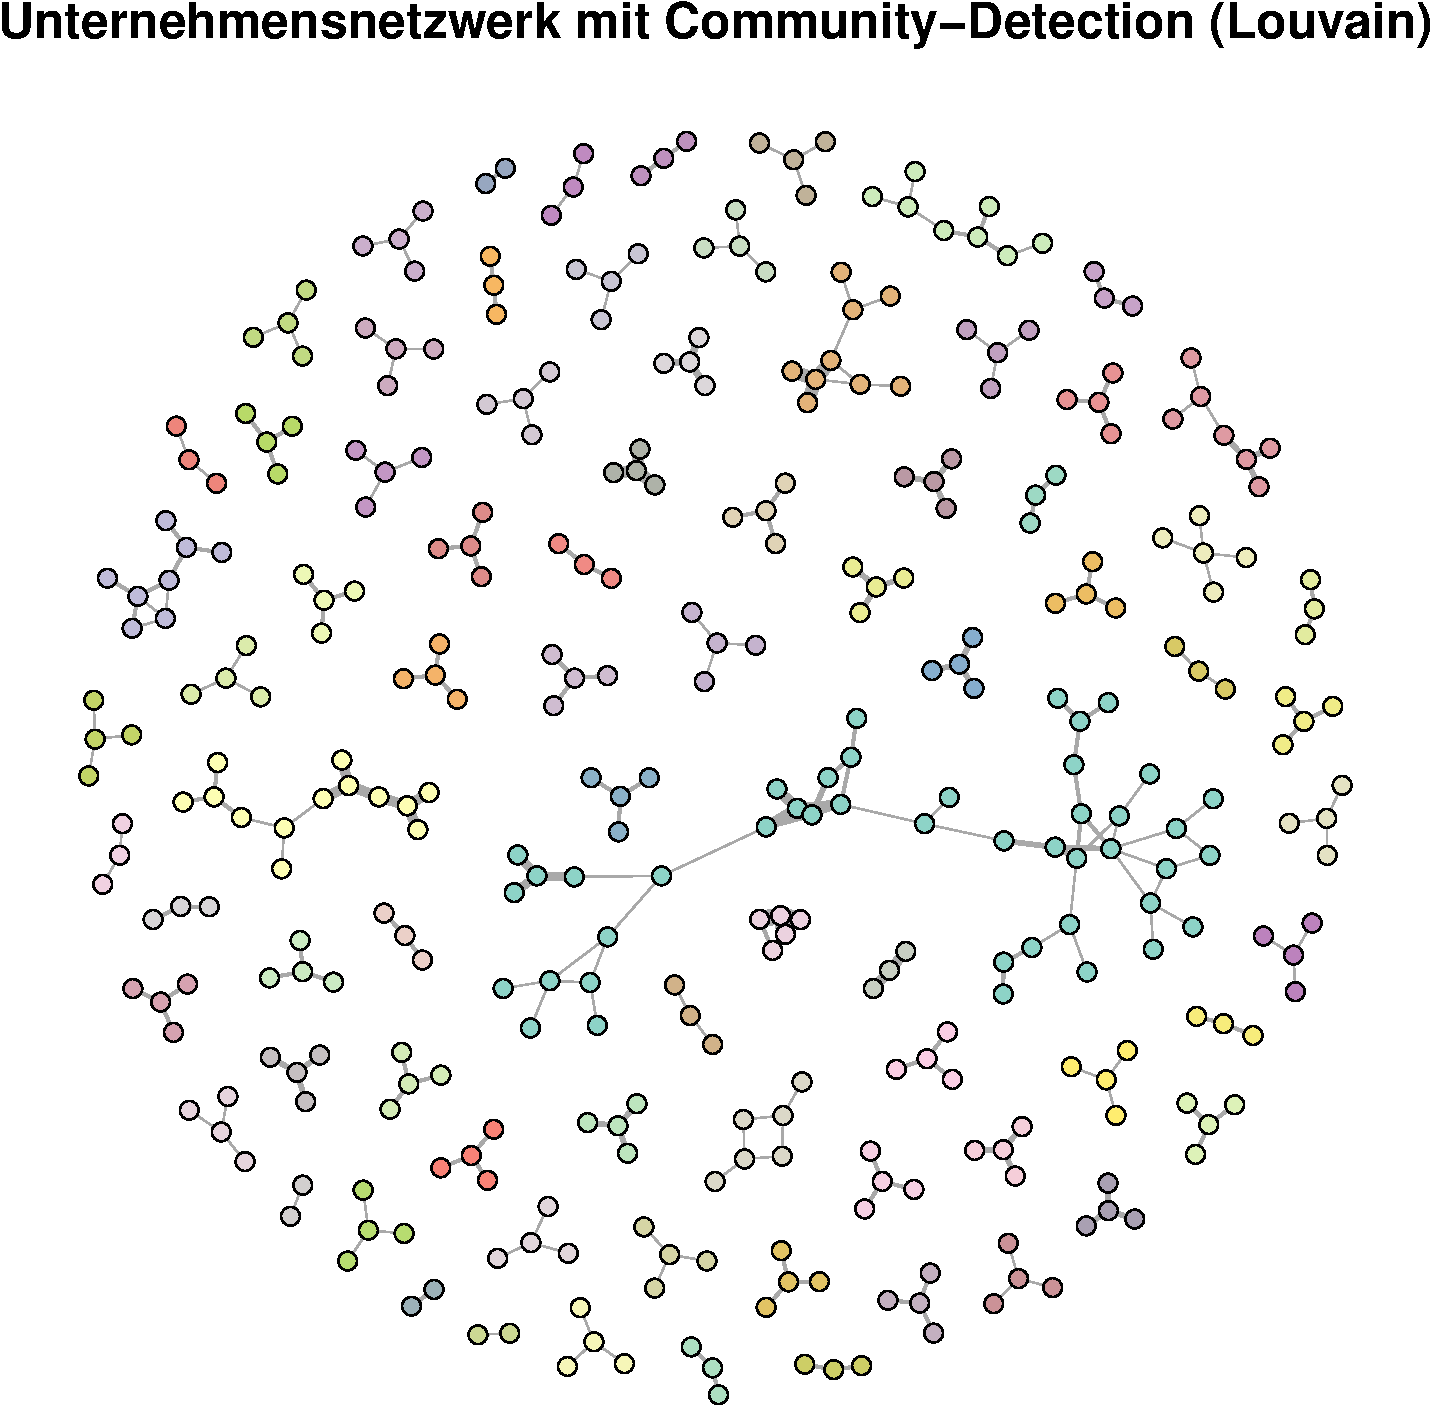
\includegraphics[keepaspectratio]{DataScience_files/figure-latex/unnamed-chunk-28-1.pdf}}
Die rote Linie zeigt einen flachen Trend ohne starke Korrelation in
diesem Scatterplot zwischen Gehalt und Degree Centrality.

Der weitgehend flache Verlauf der Trendlinie lässt den Schluss zu, dass
kein klarer Zusammenhang zwischen der Degree Centrality und den
Gehältern besteht. Dies könnte implizieren, dass die Anzahl direkter
Wettbewerber ( Degree Centrality) für sich genommen keinen signifikanten
Einfluss auf das Gehaltsniveau eines Unternehmens ausübt.

Ein kleiner Anstieg des Gehalts ist insbesondere im Bereich zwischen 100
und 150 zu verzeichnen, was darauf hindeutet, dass Unternehmen mit
mittlerem Gehaltsniveau tendenziell mehr direkte Wettbewerber haben.
Diese Entwicklung lässt sich dadurch erklären, dass Unternehmen mit
mittleren Gehaltsniveaus in stärker besetzten Märkten tätig sind, in
denen eine größere Anzahl an Unternehmen um Talente konkurriert.

Die meisten Werte der Degree Centrality sind relativ niedrig, was darauf
hindeutet, dass eine Vielzahl von Unternehmen lediglich eine geringe
Anzahl direkter Wettbewerber aufweist. Einige Unternehmen mit hoher
Degree Centrality und niedrigen bis mittleren Gehältern heben sich
jedoch von der Gesamtheit ab. Es ist möglich, dass diese Unternehmen in
stark umkämpften Märkten tätig sind, jedoch nicht über die
erforderlichen Ressourcen verfügen, um hohe Gehälter zu offerieren.

Ein Vergleich der Degree Centrality mit der Betweenness Centrality
zeigt, dass die Degree Centrality einen geringeren Einfluss auf das
Gehalt zu haben scheint. Dies lässt den Schluss zu, dass nicht die
Anzahl der direkten Wettbewerber, sondern die Position eines
Unternehmens als strategischer Vermittler im Netzwerk (Betweenness)
einflussreicher für die Höhe des Gehalts ist.

\subsubsection{Eigenvector-Zentralität}\label{eigenvector-zentralituxe4t}

Unternehmen mit hoher Eigenvector Centrality stehen nicht nur in
Konkurrenz zu einer Vielzahl von Unternehmen, sondern insbesondere zu
besonders einflussreichen Wettbewerbern im Netzwerk.

Unternehmen mit hoher Eigenvector Centrality könnten in der Konsequenz
wettbewerbsfähige Gehälter anbieten müssen, um sich im Wettbewerb mit
zentralen und attraktiven Arbeitgebern zu behaupten. Folglich sind auch
die umliegenden Firmen gezwungen, ihre Angebote anzupassen, um für die
Talente am Arbeitsmarkt attraktiv zu bleiben. Es besteht die
Möglichkeit, dass diese Unternehmen die Gehälter für spezifische,
wettbewerbsrelevante Rollen erhöhen, um den Marktstandards und den
Anforderungen eines zentralen Wettbewerbsnetzwerks gerecht zu werden.

\begin{Shaded}
\begin{Highlighting}[]
\CommentTok{\# Berechne die Eigenvector{-}Centrality und sortiere sie absteigend}
\NormalTok{top\_eigenvector }\OtherTok{\textless{}{-}} \FunctionTok{head}\NormalTok{(}\FunctionTok{sort}\NormalTok{(eigenvector\_centrality}\SpecialCharTok{$}\NormalTok{vector, }\AttributeTok{decreasing =} \ConstantTok{TRUE}\NormalTok{), }\DecValTok{5}\NormalTok{)}

\CommentTok{\# Erstelle ein DataFrame mit den Namen der Unternehmen und ihrer Eigenvector{-}Centrality}
\NormalTok{top\_eigenvector\_df }\OtherTok{\textless{}{-}} \FunctionTok{data.frame}\NormalTok{(}
  \AttributeTok{Company =} \FunctionTok{names}\NormalTok{(top\_eigenvector),}
  \AttributeTok{Eigenvector =} \FunctionTok{as.numeric}\NormalTok{(top\_eigenvector),}
  \AttributeTok{stringsAsFactors =} \ConstantTok{FALSE}
\NormalTok{)}

\CommentTok{\# Erstelle die Tabelle und zentriere sie links}
\FunctionTok{kable}\NormalTok{(top\_eigenvector\_df, }\AttributeTok{format =} \StringTok{"latex"}\NormalTok{, }\AttributeTok{booktabs =} \ConstantTok{TRUE}\NormalTok{, }\AttributeTok{align =} \StringTok{"l"}\NormalTok{) }\SpecialCharTok{\%\textgreater{}\%}
  \FunctionTok{kable\_styling}\NormalTok{(}\AttributeTok{latex\_options =} \FunctionTok{c}\NormalTok{(}\StringTok{"striped"}\NormalTok{, }\StringTok{"hold\_position"}\NormalTok{), }\AttributeTok{position =} \StringTok{"left"}\NormalTok{)}
\end{Highlighting}
\end{Shaded}

\begin{tabular}{ll}
\toprule
Company & Eigenvector\\
\midrule
\cellcolor{gray!10}{PNNL} & \cellcolor{gray!10}{1.0000000}\\
National Renewable Energy Lab & 0.5887841\\
\cellcolor{gray!10}{Oak Ridge National Laboratory} & \cellcolor{gray!10}{0.5887841}\\
Los Alamos National Laboratory & 0.5887841\\
\cellcolor{gray!10}{Pacific Northwest National Laboratory} & \cellcolor{gray!10}{0.2000000}\\
\bottomrule
\end{tabular}

\begin{Shaded}
\begin{Highlighting}[]
\CommentTok{\# Berechne die Eigenvector{-}Centrality und sortiere sie absteigend}
\NormalTok{eigenvector\_centrality }\OtherTok{\textless{}{-}} \FunctionTok{evcent}\NormalTok{(g\_competitors\_zentralität, }\AttributeTok{directed =} \ConstantTok{FALSE}\NormalTok{)}\SpecialCharTok{$}\NormalTok{vector}

\CommentTok{\# Zusammenhang zwischen durchschnittliches Gehalt und Eigenvector{-}Zentralität}
\NormalTok{salary\_eigenvector }\OtherTok{\textless{}{-}} \FunctionTok{data.frame}\NormalTok{(}
  \AttributeTok{Salary =}\NormalTok{ salary\_data}\SpecialCharTok{$}\NormalTok{AverageSalary,}
  \AttributeTok{Eigenvector =}\NormalTok{ eigenvector\_centrality[}\FunctionTok{match}\NormalTok{(salary\_data}\SpecialCharTok{$}\StringTok{\textasciigrave{}}\AttributeTok{Company Name}\StringTok{\textasciigrave{}}\NormalTok{, }\FunctionTok{names}\NormalTok{(eigenvector\_centrality))]}
\NormalTok{)}

\CommentTok{\# Entferne NA{-}Werte, die durch fehlende Übereinstimmungen entstehen könnten}
\NormalTok{salary\_eigenvector }\OtherTok{\textless{}{-}} \FunctionTok{na.omit}\NormalTok{(salary\_eigenvector)}

\CommentTok{\# Scatterplot mit roter, gestrichelter Trendlinie}
\FunctionTok{ggplot}\NormalTok{(salary\_eigenvector, }\FunctionTok{aes}\NormalTok{(}\AttributeTok{x =}\NormalTok{ Salary, }\AttributeTok{y =}\NormalTok{ Eigenvector)) }\SpecialCharTok{+}
  \FunctionTok{geom\_point}\NormalTok{() }\SpecialCharTok{+}
  \FunctionTok{geom\_smooth}\NormalTok{(}\AttributeTok{method =} \StringTok{"loess"}\NormalTok{, }\AttributeTok{se =} \ConstantTok{FALSE}\NormalTok{, }\AttributeTok{color =} \StringTok{"red"}\NormalTok{, }\AttributeTok{linetype =} \StringTok{"dashed"}\NormalTok{) }\SpecialCharTok{+}
  \FunctionTok{labs}\NormalTok{(}\AttributeTok{title =} \StringTok{"Scatterplot of Salary vs. Eigenvector Centrality"}\NormalTok{,}
       \AttributeTok{x =} \StringTok{"Salary"}\NormalTok{, }\AttributeTok{y =} \StringTok{"Eigenvector Centrality"}\NormalTok{) }\SpecialCharTok{+}
  \FunctionTok{theme\_minimal}\NormalTok{() }\SpecialCharTok{+}
  \FunctionTok{theme}\NormalTok{(}
    \AttributeTok{plot.title =} \FunctionTok{element\_text}\NormalTok{(}\AttributeTok{size =} \DecValTok{14}\NormalTok{, }\AttributeTok{face =} \StringTok{"bold"}\NormalTok{),}
    \AttributeTok{axis.title =} \FunctionTok{element\_text}\NormalTok{(}\AttributeTok{size =} \DecValTok{12}\NormalTok{, }\AttributeTok{face =} \StringTok{"bold"}\NormalTok{),}
    \AttributeTok{axis.text =} \FunctionTok{element\_text}\NormalTok{(}\AttributeTok{size =} \DecValTok{12}\NormalTok{)}
\NormalTok{  )}
\end{Highlighting}
\end{Shaded}

\begin{verbatim}
## `geom_smooth()` using formula = 'y ~ x'
\end{verbatim}

\pandocbounded{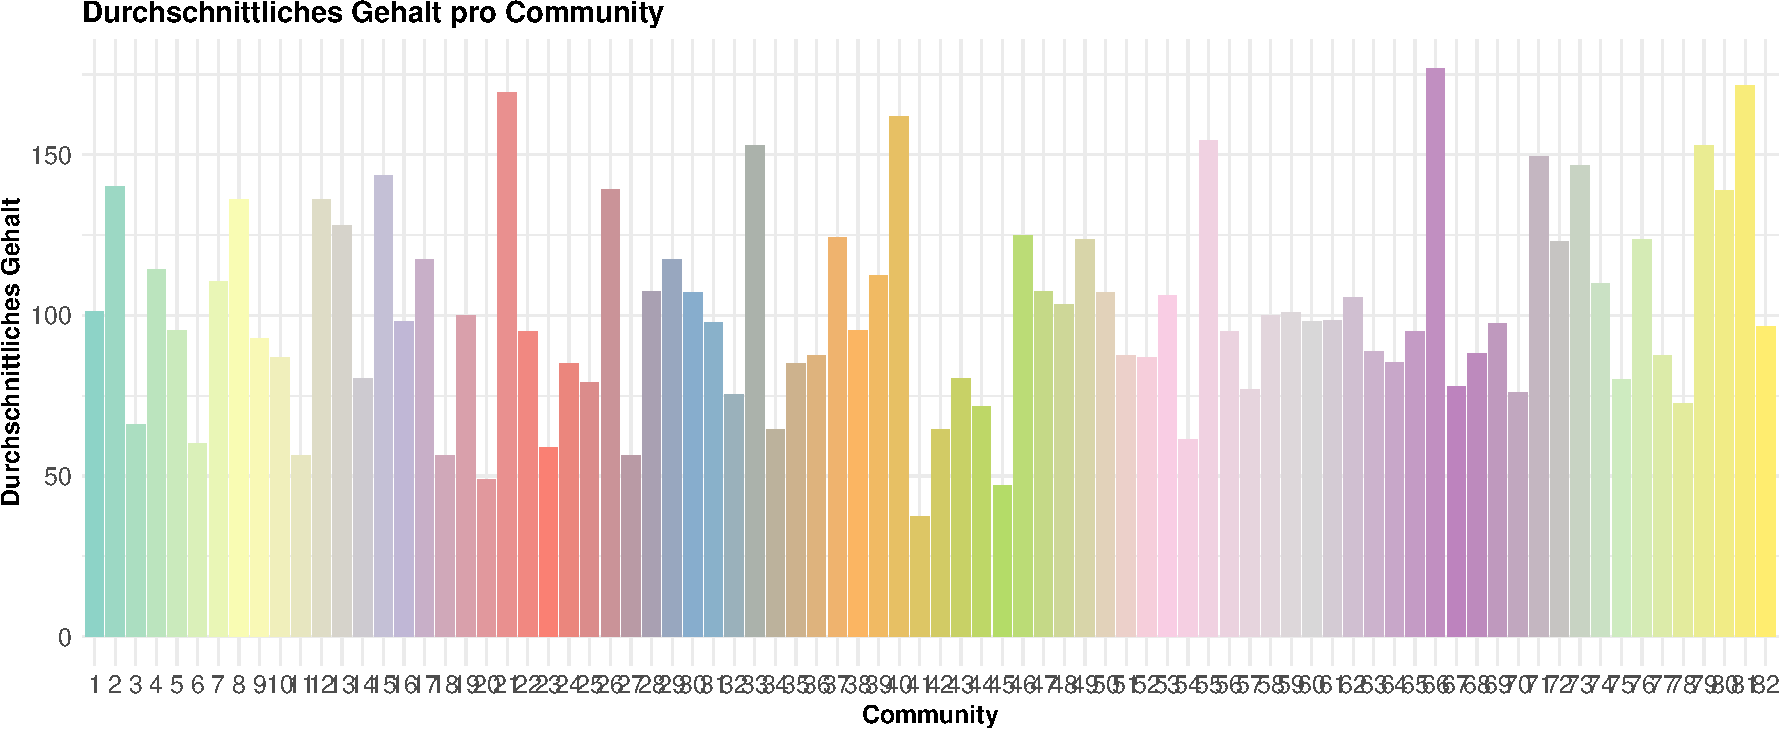
\includegraphics[keepaspectratio]{DataScience_files/figure-latex/unnamed-chunk-30-1.pdf}}

\subsection{Cluster-Analyse}\label{cluster-analyse}

Die Anwendung von Community-Detection-Methoden, wie beispielsweise
Louvain oder Walktrap, ermöglicht die Identifikation von Clustern von
Unternehmen, die sich durch einen besonders engen Wettbewerb
auszeichnen.

Im Rahmen der Klassifizierung und Visualisierung erfolgt eine farbliche
Markierung der identifizierten Cluster im Netzwerk, um eine bessere
Übersicht über die Wettbewerbsgruppen zu gewinnen.

Im Rahmen der Untersuchung wird ermittelt, ob Cluster existieren, in
denen besonders hohe oder niedrige Gehälter überwiegen, und ob diese
Cluster eine gemeinsame Markt- oder Branchenstruktur aufweisen.

\subsubsection{Clustering
Identifikation}\label{clustering-identifikation}

\begin{Shaded}
\begin{Highlighting}[]
\CommentTok{\# Louvain Community Detection}
\NormalTok{louvain\_community }\OtherTok{\textless{}{-}} \FunctionTok{cluster\_louvain}\NormalTok{(g\_direct\_competitors, }\AttributeTok{resolution =} \FloatTok{0.1}\NormalTok{)}

\CommentTok{\# Walktrap Community Detection}
\NormalTok{walktrap\_community }\OtherTok{\textless{}{-}} \FunctionTok{cluster\_walktrap}\NormalTok{(g\_direct\_competitors, }\AttributeTok{steps =} \DecValTok{2}\NormalTok{)}

\CommentTok{\# Wähle Louvain als Community{-}Detection{-}Methode}
\NormalTok{communities }\OtherTok{\textless{}{-}}\NormalTok{ louvain\_community}


\CommentTok{\# Füge die Community{-}Informationen zu den Knoten des Graphen hinzu}
\FunctionTok{V}\NormalTok{(g\_direct\_competitors)}\SpecialCharTok{$}\NormalTok{community }\OtherTok{\textless{}{-}} \FunctionTok{membership}\NormalTok{(communities)}

\CommentTok{\# Erstelle eine Farbpalette für die Communities}
\NormalTok{num\_communities }\OtherTok{\textless{}{-}} \FunctionTok{length}\NormalTok{(}\FunctionTok{unique}\NormalTok{(}\FunctionTok{V}\NormalTok{(g\_direct\_competitors)}\SpecialCharTok{$}\NormalTok{community))}
\ControlFlowTok{if}\NormalTok{ (num\_communities }\SpecialCharTok{\textgreater{}} \DecValTok{12}\NormalTok{) \{}
\NormalTok{  community\_colors }\OtherTok{\textless{}{-}} \FunctionTok{colorRampPalette}\NormalTok{(}\FunctionTok{brewer.pal}\NormalTok{(}\DecValTok{12}\NormalTok{, }\StringTok{"Set3"}\NormalTok{))(num\_communities)}
\NormalTok{\} }\ControlFlowTok{else}\NormalTok{ \{}
\NormalTok{  community\_colors }\OtherTok{\textless{}{-}} \FunctionTok{brewer.pal}\NormalTok{(num\_communities, }\StringTok{"Set3"}\NormalTok{)}
\NormalTok{\}}

\CommentTok{\# Weise die Farben den Knoten basierend auf ihrer Community zu}
\FunctionTok{V}\NormalTok{(g\_direct\_competitors)}\SpecialCharTok{$}\NormalTok{color }\OtherTok{\textless{}{-}}\NormalTok{ community\_colors[}\FunctionTok{V}\NormalTok{(g\_direct\_competitors)}\SpecialCharTok{$}\NormalTok{community]}

\CommentTok{\# Visualisiere das Netzwerk mit den Community{-}Farben}
\FunctionTok{plot}\NormalTok{(g\_direct\_competitors, }\AttributeTok{vertex.label =} \ConstantTok{NA}\NormalTok{,}
     \AttributeTok{vertex.size =} \DecValTok{3}\NormalTok{,  }\CommentTok{\# Kleinere Knoten}
     \AttributeTok{edge.width =} \DecValTok{1} \SpecialCharTok{*} \FunctionTok{E}\NormalTok{(g\_direct\_competitors)}\SpecialCharTok{$}\NormalTok{weight,  }\CommentTok{\# Reduzierte Gewichtung der Kanten}
     \AttributeTok{edge.arrow.size =} \DecValTok{1}\NormalTok{,}
     \AttributeTok{layout =}\NormalTok{ layout\_with\_fr,}
\NormalTok{)}
\FunctionTok{title}\NormalTok{(}\AttributeTok{main =} \StringTok{"Unternehmensnetzwerk mit Community{-}Detection (Louvain)"}\NormalTok{, }\AttributeTok{cex.main =} \DecValTok{2}\NormalTok{)}
\end{Highlighting}
\end{Shaded}

\pandocbounded{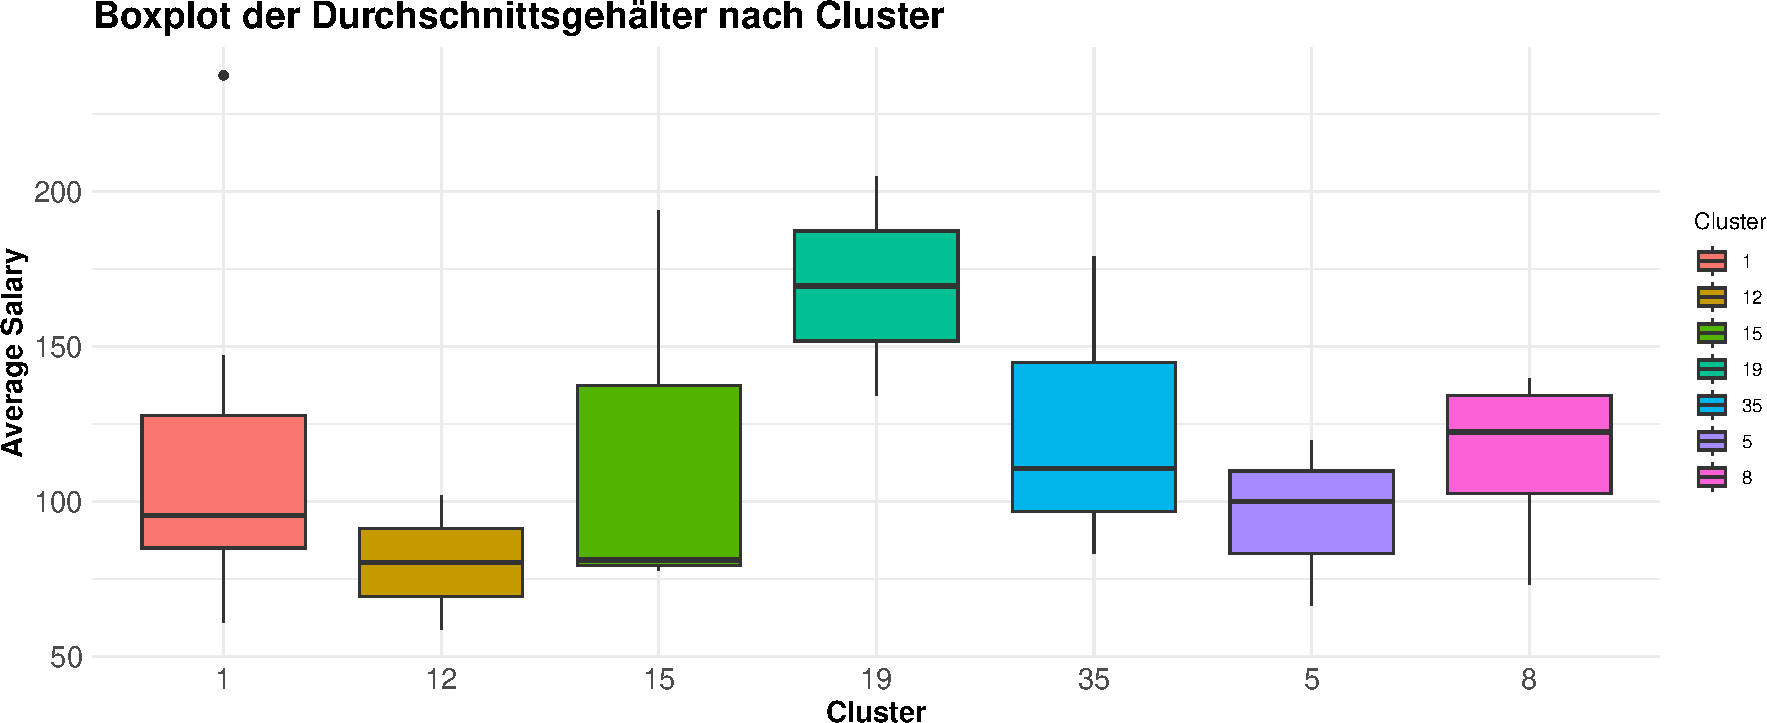
\includegraphics[keepaspectratio]{DataScience_files/figure-latex/unnamed-chunk-31-1.pdf}}

\subsubsection{Gehaltsunterschiede zwischen den
Clustern}\label{gehaltsunterschiede-zwischen-den-clustern}

\begin{Shaded}
\begin{Highlighting}[]
\CommentTok{\# Untersuche die Gehälter in den verschiedenen Clustern}
\NormalTok{community\_salary }\OtherTok{\textless{}{-}} \FunctionTok{data.frame}\NormalTok{(}
  \AttributeTok{Community =} \FunctionTok{V}\NormalTok{(g\_direct\_competitors)}\SpecialCharTok{$}\NormalTok{community,}
  \AttributeTok{Salary =} \FunctionTok{V}\NormalTok{(g\_direct\_competitors)}\SpecialCharTok{$}\NormalTok{salary}
\NormalTok{)}

\CommentTok{\# Berechne das durchschnittliche Gehalt pro Community}
\NormalTok{avg\_salary\_per\_community }\OtherTok{\textless{}{-}}\NormalTok{ community\_salary }\SpecialCharTok{\%\textgreater{}\%}
  \FunctionTok{group\_by}\NormalTok{(Community) }\SpecialCharTok{\%\textgreater{}\%}
  \FunctionTok{summarise}\NormalTok{(}\AttributeTok{AverageSalary =} \FunctionTok{mean}\NormalTok{(Salary, }\AttributeTok{na.rm =} \ConstantTok{TRUE}\NormalTok{))}

\CommentTok{\# Visualisiere die durchschnittlichen Gehälter pro Community}
\FunctionTok{ggplot}\NormalTok{(avg\_salary\_per\_community, }\FunctionTok{aes}\NormalTok{(}\AttributeTok{x =} \FunctionTok{factor}\NormalTok{(Community), }\AttributeTok{y =}\NormalTok{ AverageSalary, }\AttributeTok{fill =} \FunctionTok{factor}\NormalTok{(Community))) }\SpecialCharTok{+}
  \FunctionTok{geom\_bar}\NormalTok{(}\AttributeTok{stat =} \StringTok{"identity"}\NormalTok{) }\SpecialCharTok{+}
  \FunctionTok{scale\_fill\_manual}\NormalTok{(}\AttributeTok{values =}\NormalTok{ community\_colors) }\SpecialCharTok{+}
  \FunctionTok{labs}\NormalTok{(}\AttributeTok{title =} \StringTok{"Durchschnittliches Gehalt pro Community"}\NormalTok{,}
       \AttributeTok{x =} \StringTok{"Community"}\NormalTok{,}
       \AttributeTok{y =} \StringTok{"Durchschnittliches Gehalt"}\NormalTok{) }\SpecialCharTok{+}
  \FunctionTok{theme\_minimal}\NormalTok{() }\SpecialCharTok{+}
  \FunctionTok{theme}\NormalTok{(}
    \AttributeTok{plot.title =} \FunctionTok{element\_text}\NormalTok{(}\AttributeTok{size =} \DecValTok{14}\NormalTok{, }\AttributeTok{face =} \StringTok{"bold"}\NormalTok{),}
    \AttributeTok{axis.title =} \FunctionTok{element\_text}\NormalTok{(}\AttributeTok{size =} \DecValTok{12}\NormalTok{, }\AttributeTok{face =} \StringTok{"bold"}\NormalTok{),}
    \AttributeTok{axis.text =} \FunctionTok{element\_text}\NormalTok{(}\AttributeTok{size =} \DecValTok{12}\NormalTok{),}
    \AttributeTok{legend.position =} \StringTok{"none"}
\NormalTok{  )}
\end{Highlighting}
\end{Shaded}

\pandocbounded{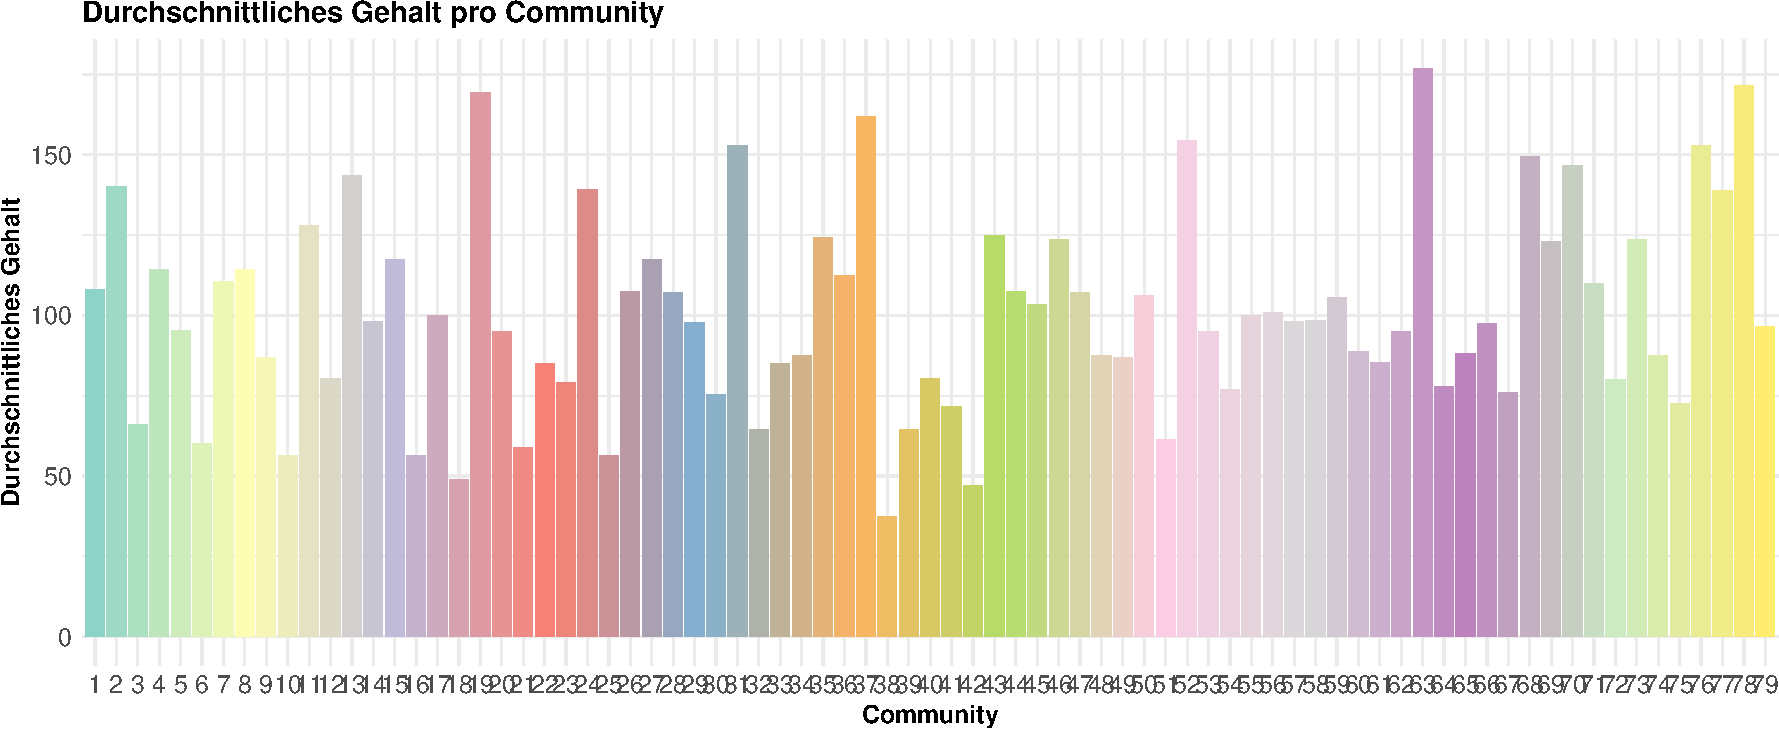
\includegraphics[keepaspectratio]{DataScience_files/figure-latex/unnamed-chunk-32-1.pdf}}

TODO ``Arc Diagramm'' zu den regionalen Clustern von der geografischen
Netzwerkanalyse

\subsection{Zurückbesinnen auf die geografische
Analyse?}\label{zuruxfcckbesinnen-auf-die-geografische-analyse}

\section{Abschließende Betrachtung mittels interaktiver
Visualisierung}\label{abschlieuxdfende-betrachtung-mittels-interaktiver-visualisierung}

\begin{Shaded}
\begin{Highlighting}[]
\NormalTok{closeness\_centrality }\OtherTok{\textless{}{-}} \FunctionTok{closeness}\NormalTok{(g\_direct\_competitors)}
\NormalTok{clustering\_coeff }\OtherTok{\textless{}{-}} \FunctionTok{transitivity}\NormalTok{(g\_direct\_competitors, }\AttributeTok{type =} \StringTok{"local"}\NormalTok{)}
\end{Highlighting}
\end{Shaded}

\begin{Shaded}
\begin{Highlighting}[]
\CommentTok{\# Prepare data for visNetwork}
\StringTok{\textquotesingle{}nodes \textless{}{-} data.frame(id = V(g\_direct\_competitors)$name,}
\StringTok{                    label = V(g\_direct\_competitors)$name,}
\StringTok{                    group = membership(communities),}
\StringTok{                    value = degree\_centrality,}
\StringTok{                    title = paste("Degree:", degree\_centrality, }
\StringTok{                                  "\textless{}br\textgreater{}Betweenness:", betweenness\_centrality,}
\StringTok{                                  "\textless{}br\textgreater{}Closeness:", closeness\_centrality,}
\StringTok{                                  "\textless{}br\textgreater{}Eigenvector:", eigenvector\_centrality))}

\StringTok{edges \textless{}{-} data.frame(from = as.character(edges$from), to = as.character(edges$to))}

\StringTok{\# Create interactive network visualization}
\StringTok{visNetwork(nodes, edges) \%\textgreater{}\%}
\StringTok{  visOptions(highlightNearest = TRUE, nodesIdSelection = TRUE) \%\textgreater{}\%}
\StringTok{  visGroups(groupname = "1", color = "red") \%\textgreater{}\%}
\StringTok{  visGroups(groupname = "2", color = "blue") \%\textgreater{}\%}
\StringTok{  visGroups(groupname = "3", color = "green") \%\textgreater{}\%}
\StringTok{  visGroups(groupname = "4", color = "yellow") \%\textgreater{}\%}
\StringTok{  visGroups(groupname = "5", color = "purple") \%\textgreater{}\%}
\StringTok{  visGroups(groupname = "6", color = "orange") \%\textgreater{}\%}
\StringTok{  visGroups(groupname = "7", color = "pink") \%\textgreater{}\%}
\StringTok{  visLayout(randomSeed = 123) \%\textgreater{}\%}
\StringTok{  visLegend()\textquotesingle{}}
\end{Highlighting}
\end{Shaded}

\begin{verbatim}
## [1] "nodes <- data.frame(id = V(g_direct_competitors)$name,\n                    label = V(g_direct_competitors)$name,\n                    group = membership(communities),\n                    value = degree_centrality,\n                    title = paste(\"Degree:\", degree_centrality, \n                                  \"<br>Betweenness:\", betweenness_centrality,\n                                  \"<br>Closeness:\", closeness_centrality,\n                                  \"<br>Eigenvector:\", eigenvector_centrality))\n\nedges <- data.frame(from = as.character(edges$from), to = as.character(edges$to))\n\n# Create interactive network visualization\nvisNetwork(nodes, edges) %>%\n  visOptions(highlightNearest = TRUE, nodesIdSelection = TRUE) %>%\n  visGroups(groupname = \"1\", color = \"red\") %>%\n  visGroups(groupname = \"2\", color = \"blue\") %>%\n  visGroups(groupname = \"3\", color = \"green\") %>%\n  visGroups(groupname = \"4\", color = \"yellow\") %>%\n  visGroups(groupname = \"5\", color = \"purple\") %>%\n  visGroups(groupname = \"6\", color = \"orange\") %>%\n  visGroups(groupname = \"7\", color = \"pink\") %>%\n  visLayout(randomSeed = 123) %>%\n  visLegend()"
\end{verbatim}

\begin{Shaded}
\begin{Highlighting}[]
\CommentTok{\# Fügt ein Bild der interaktiven Netzwerkvisualisierung hinzu}
\CommentTok{\# knitr::include\_graphics("interaktive\_Netzwerke\_Bilder/Übersicht.png")}

\CommentTok{\# knitr::include\_graphics("interaktive\_Netzwerke\_Bilder/NVDIA.png")}
\end{Highlighting}
\end{Shaded}

Zugriff auf die interaktive Visualisierung über das Repository
(Dateiname: network.html): \url{https://github.com/Mzaex7/SNA}

\newpage

\section{Conclusion}\label{conclusion}

Zusammenfassung der Ergebnisse: Fasse die zentralen Erkenntnisse zur
Rolle des Wettbewerbs im Gehaltsgefüge von Data Science-Positionen
zusammen, wie etwa: „Unternehmen in Clustern mit hoher
Degree-Zentralität bieten im Durchschnitt 15 \% höhere Gehälter als
isolierte Unternehmen.``

Bedeutung der Ergebnisse: Diskutiere die Bedeutung der
Wettbewerbsstruktur und welche Unternehmen durch ihre Position im
Netzwerk von Wettbewerbsvorteilen und Talentrekrutierung profitieren.

Praktische Empfehlungen: Leite Handlungsempfehlungen für
Berufseinsteiger und Unternehmen ab: Wo und wie sollten Fachkräfte ihre
Karrieresuche fokussieren? Welche Unternehmen sollten strategische
Investitionen in Gehälter und Talentförderung in Erwägung ziehen?

\newpage

\section{Literaturverzeichnis}\label{literaturverzeichnis}

Davenport, Thomas H.; Patil, D. J. 2012. »Data Scientist: The Sexiest
Job of the 21st Century«, in Harvard Business Review vom 1. Oktober
2012.
\url{https://hbr.org/2012/10/data-scientist-the-sexiest-job-of-the-21st-century}
(Zugriff vom 30.10.2024).

Google Trends,
\url{https://trends.google.com/trends/explore?date=all&q=\%22data\%20science\%22,\%22data\%20scientist\%22}
(Zugriff vom 30.10.2024).

\end{document}
